%%%%%%%%%%%%%%%%%%%%%%%%%%%%%%%%%%%%%%%%%
% Daily Laboratory Book
% LaTeX Template
% Version 1.0 (4/4/12)
%
% This template has been downloaded from:
% http://www.LaTeXTemplates.com
%
% Original author:
% Frank Kuster (http://www.ctan.org/tex-archive/macros/latex/contrib/labbook/)
%
% Important note:
% This template requires the labbook.cls file to be in the same directory as the
% .tex file. The labbook.cls file provides the necessary structure to create the
% lab book.
%
% The \lipsum[#] commands throughout this template generate dummy text
% to fill the template out. These commands should all be removed when 
% writing lab book content.
%
% HOW TO USE THIS TEMPLATE 
% Each day in the lab consists of three main things:
%
% 1. LABDAY: The first thing to put is the \labday{} command with a date in 
% curly brackets, this will make a new page and put the date in big letters 
% at the top.
%
% 2. EXPERIMENT: Next you need to specify what experiment(s) you are 
% working on with an \experiment{} command with the experiment shorthand 
% in the curly brackets. The experiment shorthand is defined in the 
% 'DEFINITION OF EXPERIMENTS' section below, this means you can 
% say \experiment{pcr} and the actual text written to the PDF will be what 
% you set the 'pcr' experiment to be. If the experiment is a one off, you can 
% just write it in the bracket without creating a shorthand. Note: if you don't 
% want to have an experiment, just leave this out and it won't be printed.
%
% 3. CONTENT: Following the experiment is the content, i.e. what progress 
% you made on the experiment that day.
%
%%%%%%%%%%%%%%%%%%%%%%%%%%%%%%%%%%%%%%%%%

%----------------------------------------------------------------------------------------
%	PACKAGES AND OTHER DOCUMENT CONFIGURATIONS
%----------------------------------------------------------------------------------------

\documentclass[idxtotoc,hyperref,openany]{labbook} % 'openany' here removes the gap page between days, erase it to restore this gap; 'oneside' can also be added to remove the shift that odd pages have to the right for easier reading

\usepackage{tikz}
\usepackage[table,xcdraw]{xcolor}
\usepackage{colortbl}

\usepackage[ 
  backref=page,
  pdfpagelabels=true,
  plainpages=false,
  colorlinks=true,
  bookmarks=true,
  pdfview=FitB]{hyperref} % Required for the hyperlinks within the PDF
  
\usepackage{booktabs} % Required for the top and bottom rules in the table
\usepackage{float} % Required for specifying the exact location of a figure or table
\usepackage{graphicx} % Required for including images2
\usepackage{lipsum} % Used for inserting dummy 'Lorem ipsum' text into the template
\usepackage[shortlabels]{enumitem}
\usepackage{pgfplots, pgfplotstable}
\usepackage{siunitx}

\newcommand{\HRule}{\rule{\linewidth}{0.5mm}} % Command to make the lines in the title page
\setlength\parindent{0pt} % Removes all indentation from paragraphs

%----------------------------------------------------------------------------------------
%	DEFINITION OF EXPERIMENTS
%----------------------------------------------------------------------------------------

\newexperiment{example}{This is an example experiment}
\newexperiment{example2}{This is another example experiment}
\newexperiment{example3}{This is yet another example experiment}
\newexperiment{table}{This shows a sample table}
%\newexperiment{shorthand}{Description of the experiment}

%---------------------------------------------------------------------------------------

\begin{document}

%----------------------------------------------------------------------------------------
%	TITLE PAGE
%----------------------------------------------------------------------------------------

\frontmatter % Use Roman numerals for page numbers
\title{
\begin{center}
\HRule \\[0.4cm]
{\Huge \bfseries Laboratory Journal \\[0.5cm] \Large Bachelor of Science}\\[0.4cm] % Degree
\HRule \\[1.5cm]
\end{center}
}
\author{\Huge Tiffany Pham \\ \\ \LARGE tpham118@ucmerced.edu \\[2cm]} % Your name and email address
\date{Beginning 27 January 2025} % Beginning date
\maketitle

\tableofcontents

\mainmatter % Use Arabic numerals for page numbers

%----------------------------------------------------------------------------------------
%	LAB BOOK CONTENTS
%----------------------------------------------------------------------------------------

% Blank template to use for new days:

%\labday{Day, Date Month Year}

%\experiment{}

%Text

%-----------------------------------------

%\experiment{}

%Text

%----------------------------------------------------------------------------------------

\labday{Monday, 27 January 2025}
\vspace{-5mm}
Tiffany Pham

\experiment{Lab 01 (Lab) - Lab Notebook Analysis}
\textbf{Purpose}

The purpose of this lab is to evaluate the completeness and effectiveness of my lab notebook as a standalone record of past experiments. This includes determining whether previous entries provide sufficient detail to replicate an experiment, identifying errors or inconsistencies, and assessing my ability to achieve learning objectives through proper documentation.

\hfill \break
\textbf{Objective(s)}
\begin{enumerate}[$\bullet$]
    \item Assess the completeness of recorded experiments and their reproducibility.
    \item Identify mistakes or gaps in documentation and understand how they impact results.
    \item Apply the lab notebook checklist to self-evaluate my record-keeping.
    \item Recognize strengths and areas for improvement in lab documentation.
\end{enumerate}

\hfill \break
\textbf{Equipment needed}
\begin{enumerate}[$\bullet$]
    \item Two previous Phys 8L lab notebook entries (Lab 03: Logger Pro \& Lab 05: Force Sensor Lab).
    \item Lab Notebook Guide.
    \item Lab Notebook Checklist Rubric.
\end{enumerate}

\hfill \break
\textbf{Experimental Plan/Procedure}
\begin{enumerate}
    \item Without referring to the lab manual, attempt to determine if I can repeat past experiments based solely on my lab notebook entries.
    \item Identify errors, missing details, or unclear steps that would make replication difficult.
    \item Compare past recorded data to expected results and assess if the documentation is sufficient.
    \item Analyze lab objectives and determine if my records show their achievement.
    \item Reflect on personal strengths and weaknesses in maintaining a lab notebook.
    \item Identify areas where TA feedback would be most helpful.
\end{enumerate}

%----------------------------------------------------------------------------------------

\experiment{Carrying Out the Experiment (Lab Notebook Answers)} % Multiple experiments can be included in a single day, this allows you to segment what was done each day into separate categories
\begin{enumerate}
    \item The first lab notebook I used was Lab 03 - Logger Pro and Lab 05 - Force Sensor lab. Without looking at the associated lab manual and each lab notebook, I can repeat the experiment based on what was recorded in the lab notebook. The information that I found helpful was on how to set up the track, cart, and force sensor to get her with all the necessary attachments. However, I could have been more thorough with the instructions, such as including a picture of the workstation with all the labels needed, which would have helped make my procedure much more straightforward.
    \item Looking through my lab notebook, I do not have these types of situations often, but when I do, I usually have an error in the graph or the data I collected. For example, for Lab 03 - Logger Pro, the data that I collected did not make sense at all. The data had too many sudden fluctuations and too many rectangle-shaped shapes. The ideal data are supposed to look smooth and not have sudden fluctuations; otherwise, it would seem as if the cart teleported or traveled way too fast. But yes, if I have instances like these, it is easy to identify these situations since I would explain them in my data and/or notes.
    \item Regarding the Lab Objectives, I would have them in most lab notebooks. I noticed I have two lab notebooks with no objectives, but everything else has the objectives. The ones that have the lab objectives, I can tell that I have achieved each of the lab's objectives. I showed the steps and what I did in each lab. Then, I explain and observe the data and explain how and why it relates to the lab's objectives.
    \item Reviewing Lab notebook:
    \begin{enumerate}[(a)]
        \item I think my strength is the way I wrote the procedures. I made sure to make it detailed and include as much data as possible from what I did. I would always try to make it easy to follow and explain the steps as quickly and clearly as possible.
        \item I think the areas I need the most practice are remembering to write the lab objectives and the reflections on my data. I would have the lab objectives and reflections in some lab notebooks, but I would often forget to include them. I wish I had gone back to my lab notebooks and taken the time to ensure I included as much information as possible because now, reading back on them, there are times when comprehending them is difficult.
        \item I think the feedback where I find most helpful is telling me if I am missing some integral parts of the lab notebook. Sometimes, I forget certain parts of the lab notebook, and I would find it helpful if the TA pointed it out if it were to happen.
        \item Not applicable. I do not have any questions so far.
    \end{enumerate}
    \item Based on this lab's learning objectives, I think I have achieved them because I was able to determine how thorough my lab notebook is as a standalone record of the associated lab, reference the lab notebook rubric, and apply accurate ratings to my work, explain how misunderstandings and mistakes in the experimental process assist in learning, and identify my strengths and weaknesses in keeping a lab notebook. I was able to achieve all these through the lab notebook prompts that I answered.
\end{enumerate}

%----------------------------------------------------------------------------------------

\experiment{Conclusion}
This lab provided an important \textbf{self-assessment} of my lab notebook practices. I identified several areas for improvement, particularly in \textbf{data annotation, predictions, and reflections}. Moving forward, I will focus on making my lab notes \textbf{more comprehensive and reproducible} by including \textbf{better annotations, labeled images, and explicit data interpretations}.

%----------------------------------------------------------------------------------------

\vspace{-5mm}
\labday{Monday, 03 February 2025}
\vspace{-5mm}
Tiffany Pham

\experiment{Lab 02 (Lab) - Phyphox Intro}
\textbf{Purpose}

The purpose of this lab is to introduce the use of the \textbf{Phyphox} app for data collection, visualization, and analysis. This includes understanding how to collect and export data, interpret motion along different axes, and apply annotation and zooming functions within the app.

\hfill \break
\textbf{Objective(s)}
\begin{enumerate}[$\bullet$]
    \item Apply skills from Lab 01 to maintain an effective lab notebook.
    \item Collect and analyze data using the \textbf{Phyphox app}.
    \item Differentiate between \textbf{1D and multi-dimensional motion}.
    \item Determine the \textbf{x-, y-, and z-axes} of my smartphone.
    \item Learn to \textbf{annotate, zoom, and extract specific data} points from recorded datasets.
    \item Export and organize data for future reference.
\end{enumerate}

\hfill \break
\textbf{Equipment needed}
\begin{enumerate}[$\bullet$]
    \item \textbf{Smartphone} with Phyphox installed.
    \item \textbf{Phyphox App Features:}
    \begin{enumerate}[$\bullet$]
        \item Acceleration (without g) sensor.
        \item Gyroscope (rotation rate) sensor.
    \end{enumerate}
    \item Computer for exporting and analyzing data.
\end{enumerate}

\hfill \break
\textbf{Experimental Plan/Procedure}
\begin{enumerate}
    \item \textbf{Collect acceleration data} using the "Acceleration (without g)" sensor with a motion different from the example shown in the slides.
    \item \textbf{Describe the phone’s motion} and determine whether it is \textbf{1D or multi-dimensional}.
    \item \textbf{Repeat the motion multiple times}, ensuring that most movement is along a single axis.
    \item \textbf{Annotate a screenshot} of the main data view, marking key points.
    \item \textbf{Use different data views}: pan, zoom, and pick a data point.
    \item \textbf{Extract data points and find acceleration differences}, using the "pick data" function.
    \item \textbf{Export a dataset to the computer}, record the filename and location.
    \item \textbf{Use the Gyroscope sensor} to determine the phone’s axes (x, y, z) and verify them with experimental data.
\end{enumerate}

%----------------------------------------------------------------------------------------

\experiment{Carrying Out the Experiment}

\textbf{Collecting Acceleration Data (Without g)}
\begin{enumerate}[$\bullet$]
    \item \textbf{Motion Performed}: Phone was dropped onto the table, resulting in a couple of bounces.
    \item \textbf{1D Confirmation}: Data was primarily recorded in the \textbf{linear acceleration z-axis}, where noticeable spikes occurred during each bounce, followed by a return to baseline values.
    \item \textbf{Factors for Clean Data:}
    \begin{itemize}[$\bullet$]
        \item Smooth, consistent motion.
        \item Reducing external vibrations.
        \item Ensuring minimal hand movement in unintended directions.
    \end{itemize}
    \item \textbf{Screenshots taken:} One showing \textbf{raw acceleration data} (see figure \ref{fig:Lab02-PhoneDropFull1}) and another with \textbf{annotated points} (see figure \ref{fig:Lab02-PhoneDropZAnnotated1}) for reference.
\end{enumerate}
\textbf{Annotating the Data View}
\begin{enumerate}[$\bullet$]
    \item \textbf{Added labels and marks} on the main screen to highlight acceleration peaks.
    \item Included a \textbf{simple annotation} (e.g., a smiley face) to demonstrate knowledge of the function.
    \item View figure \ref{fig:Lab02-Annotated} for proof.
\end{enumerate}
\newpage
\textbf{Exploring Different Data Views}
\begin{enumerate}[$\bullet$]
    \item \textbf{Enlarged x-, y-, and z-axis plots} to analyze differences. (View figures \ref{fig:Lab02-PhoneDropX}, \ref{fig:Lab02-PhoneDropY}, \ref{fig:Lab02-PhoneDropZ} for proof)
    \item Practiced \textbf{panning and zooming} to focus on specific time intervals. (View figures \ref{fig:Lab02-PhoneDropZzoomed}, \ref{fig:Lab02-PhoneDropZAnnotated1}, \ref{fig:Lab02-PhoneDropZAnnotated2} for proof.
    \item \textbf{Selected specific data points} and calculated acceleration differences.
    \begin{enumerate}[$\bullet$]
        \item \textbf{Largest difference recorded: 160.1 m/s$^2$} in z-axis acceleration.
        \item View figures \ref{fig:Lab02-PhoneDropZAnnotated1}, \ref{fig:Lab02-PhoneDropZAnnotated2}, \ref{fig:Lab02-PhoneDropZAnnotated3}, \ref{fig:Lab02-PhoneDropZAnnotated4} for proof.
    \end{enumerate}
\end{enumerate}
\textbf{Exporting and Recording Data}
\begin{enumerate}[$\bullet$]
    \item \textbf{Data set exported:} "AccelerationWithoutG\textunderscore 2025-02-03 18-22-45.xls"
    \item File Location: Physics 9L $>$ Lab02\textunderscore Data
    \item \textbf{Metadata recorded:} 
    \begin{enumerate}[$\bullet$]
        \item \textbf{Phyphox sensor used:} Acceleration without g.
        \item \textbf{Description of motion:} Phone was dropped onto table 5 inches above it.
        \item \textbf{Timestamp}: 18:23
    \end{enumerate}
    \item \textbf{Data Point Count:} 830 points.
    \item \textbf{Timestep Between Points: 0.01s}
    \item View figure \ref{fig:Lab02-PhoneDropDataSet} for proof.
\end{enumerate}
\textbf{Determining the Phone’s Axes}
\begin{enumerate}[$\bullet$]
    \item Using the Gyroscope sensor:
    \begin{enumerate}[$\bullet$]
        \item Rotated phone counterclockwise, identifying the \textbf{z-axis direction}.
        \item Tilted phone sideways to determine the \textbf{y-axis direction}.
        \item Tilted phone forward/backward to determine the \textbf{x-axis direction}.
    \end{enumerate}
    \item \textbf{Results:}
    \begin{enumerate}[$\bullet$]
        \item \textbf{X-axis:} Points left/right when holding phone upright.
        \item \textbf{Y-axis:} Points up/down.
        \item \textbf{Z-axis:} Points out of the screen.
    \end{enumerate}
    \item View figures \ref{fig:Lab02-GyroscopeX}, \ref{fig:Lab02-GyroscopeY}, \ref{fig:Lab02-GyroscopeZ} for proof.
\end{enumerate}

%----------------------------------------------------------------------------------------

\experiment{Data Analysis}
In each gyroscope recording, I could tell whether it was the x, y, or z axis because one of the graphs (x, y, or z) would stand out the most, for example, on all the data on the left-hand side. One of the graphs would stand out the most, meaning it would have more recorded data sets than all the others. That was how I figured out what axis my phone was recording based on the datasets provided.

%----------------------------------------------------------------------------------------

\experiment{Data Interpretation}
\begin{enumerate}[$\bullet$]
    \item \textbf{1D Motion was verified} since acceleration was mainly recorded along one axis at a time.
    \item \textbf{Data processing skills improved} by using pan, zoom, and pick data point tools.
    \item \textbf{Exporting data and recording metadata ensured reproducibility.}
    \item \textbf{Gyroscope results confirmed correct phone axis identification.}
\end{enumerate}

%----------------------------------------------------------------------------------------

\experiment{Achievement of Learning Objectives}
\begin{enumerate}[$\bullet$]
    \item \checkmark \hspace{1mm} Successfully \textbf{collected and analyzed} data using Phyphox.
    \item \checkmark \hspace{1mm} Used different views (main screen, zoom, pan, pick data).
    \item \checkmark \hspace{1mm} Determined \textbf{phone’s x-, y-, and z-axes} using Gyroscope sensor.
    \item \checkmark \hspace{1mm} Exported data properly and recorded necessary details.
\end{enumerate}

%----------------------------------------------------------------------------------------

\experiment{Conclusion}
This lab introduced \textbf{Phyphox as a data collection tool}, providing hands-on experience with \textbf{acceleration and gyroscope sensors}. The data collected successfully demonstrated \textbf{1D motion}, and I gained experience with \textbf{zooming, panning, and annotating data}. Moving forward, I will focus on \textbf{improving data visualization and exploring multi-dimensional motion} in later labs.

%----------------------------------------------------------------------------------------

\newpage
\experiment{Data Pictures}
\textbf{Collecting Acceleration Data (Without g)}
\begin{figure}[H] % Example of including images
\begin{center}
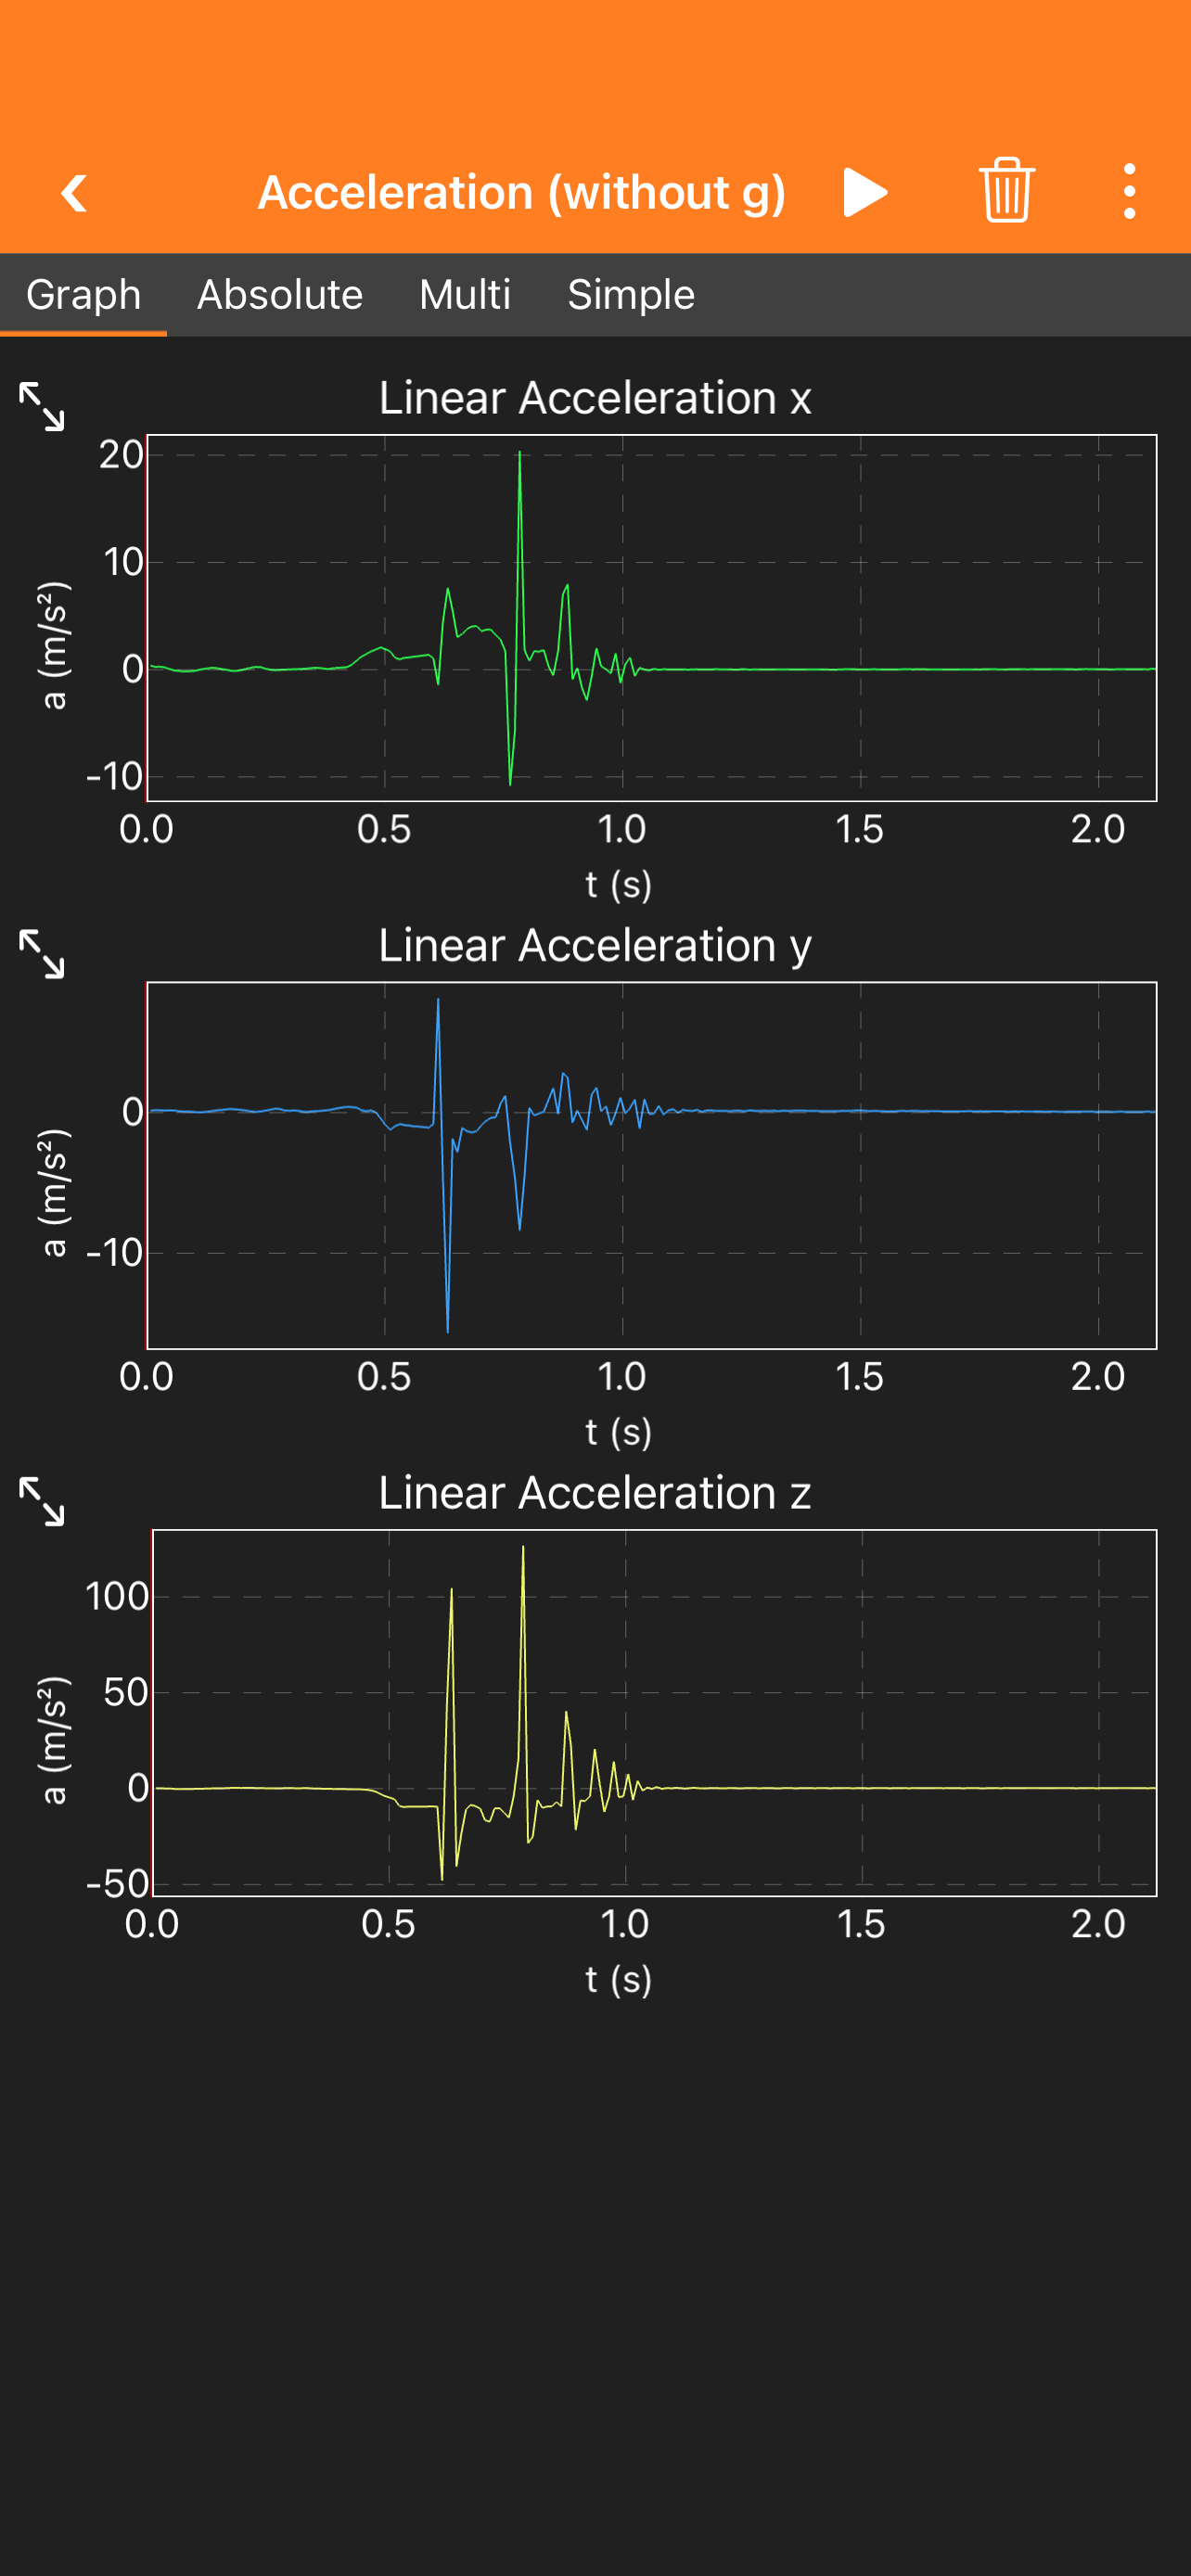
\includegraphics[width=.55\linewidth]{images/Lab.02/PhoneDropFull1.PNG}
\end{center}
\caption{Full screenshot of the raw acceleration data}
\label{fig:Lab02-PhoneDropFull1}
\end{figure}

\begin{figure}[H] % Example of including images
\begin{center}
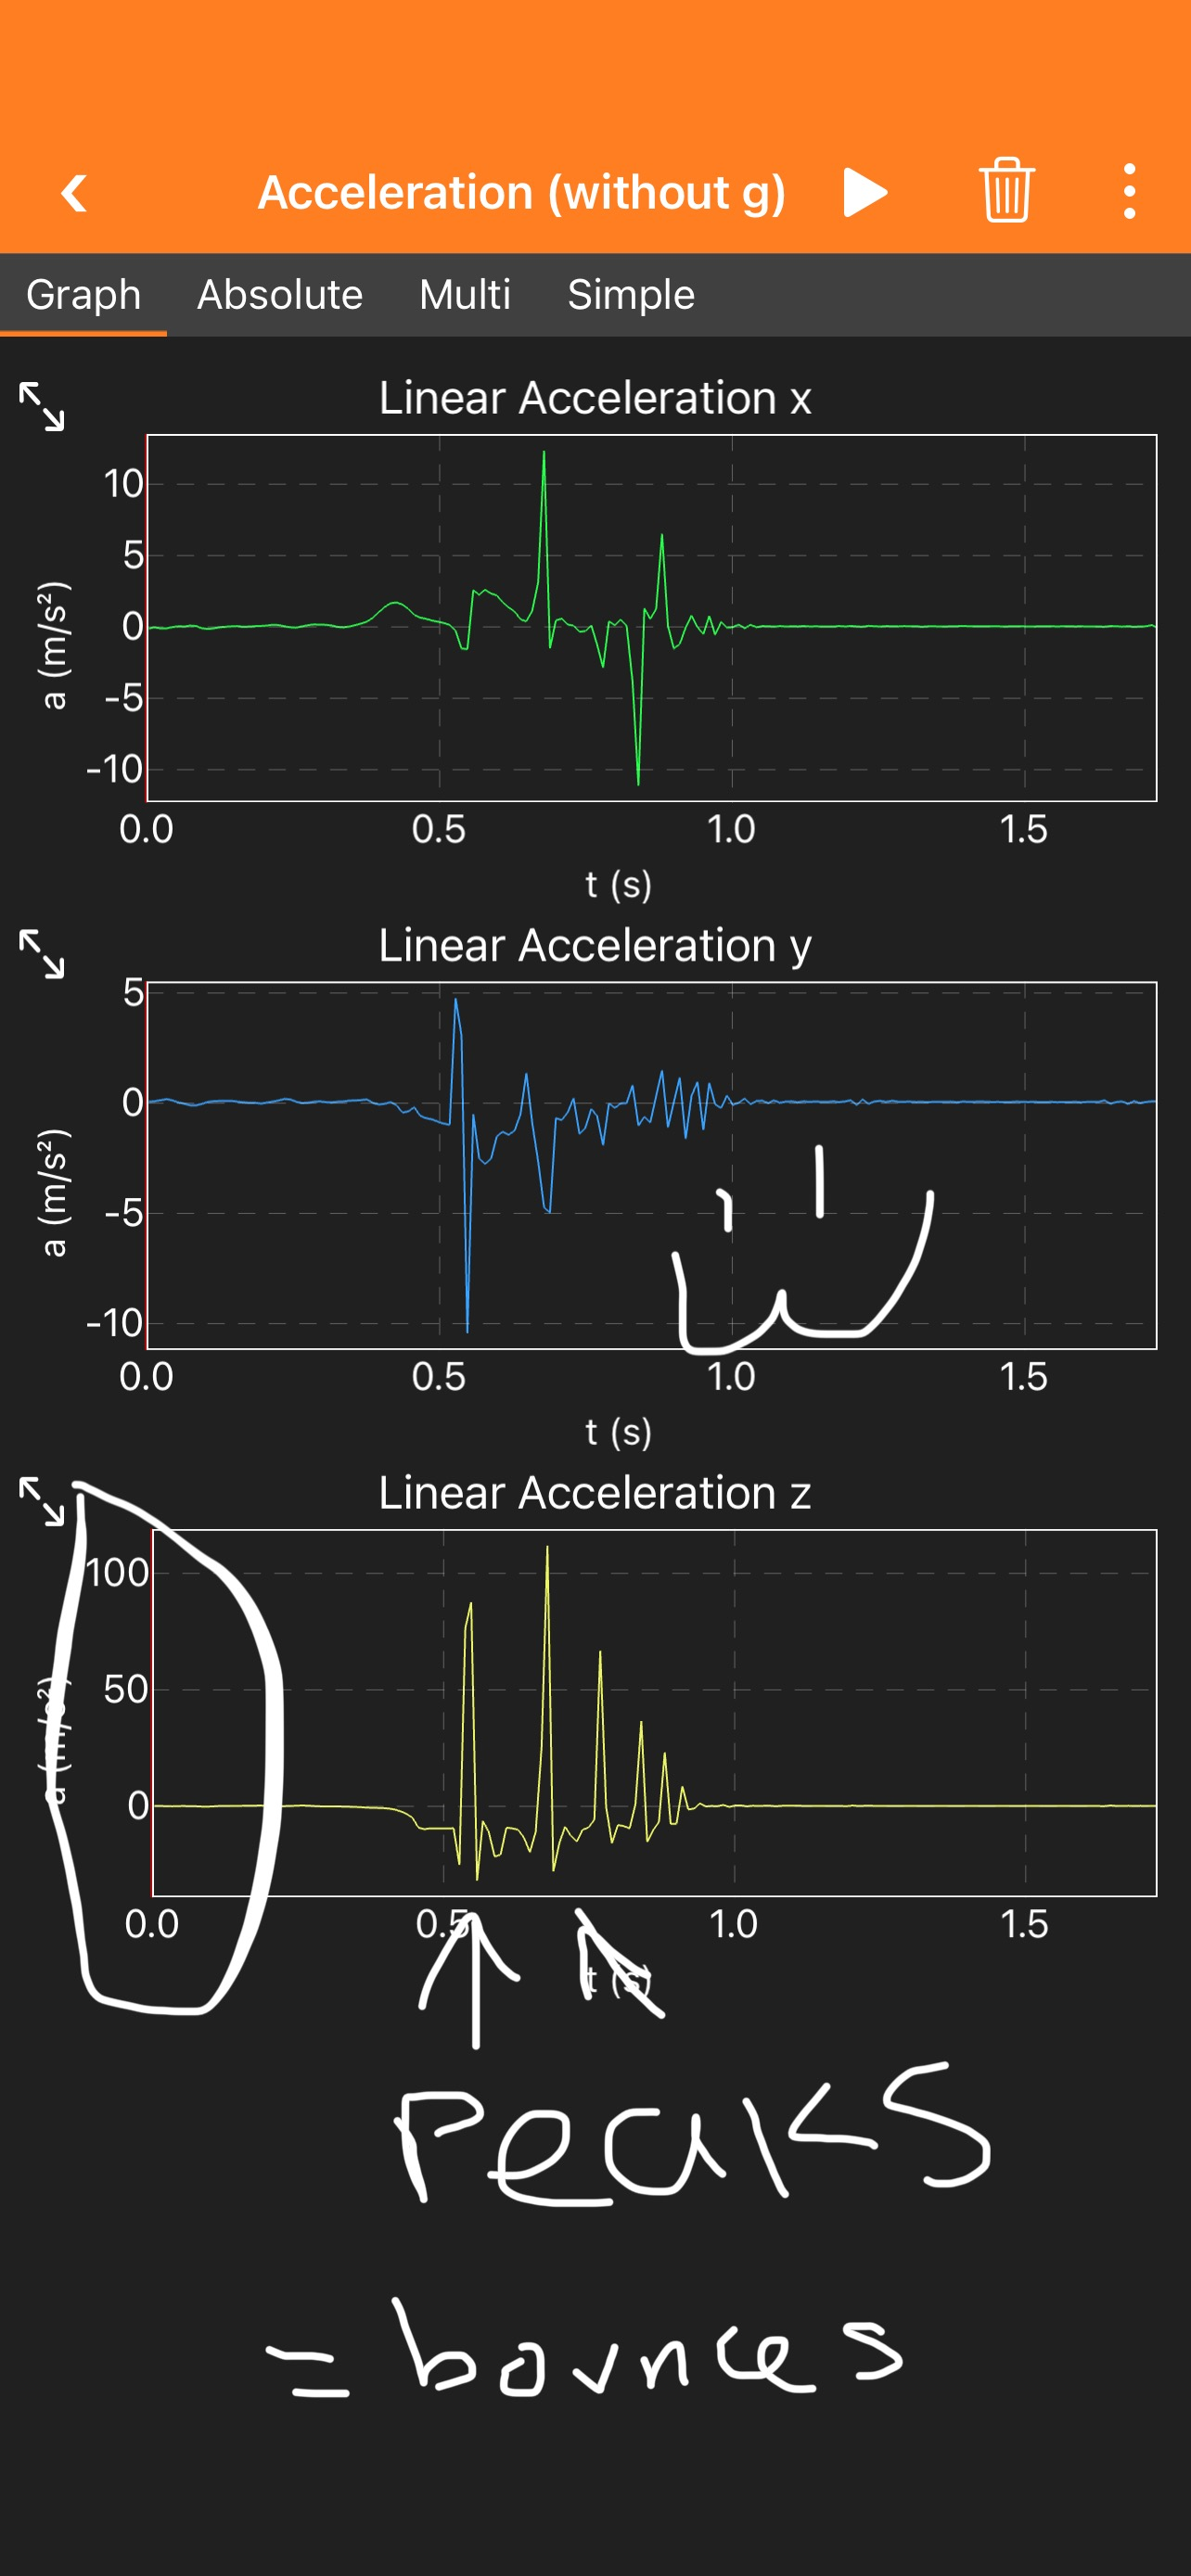
\includegraphics[width=.7\linewidth]{images/Lab.02/Annotated.jpg}
\end{center}
\caption{Screenshot of a graph with annotations and smiley face.}
\label{fig:Lab02-Annotated}
\end{figure}

\begin{figure}[H] % Example of including images
\begin{center}
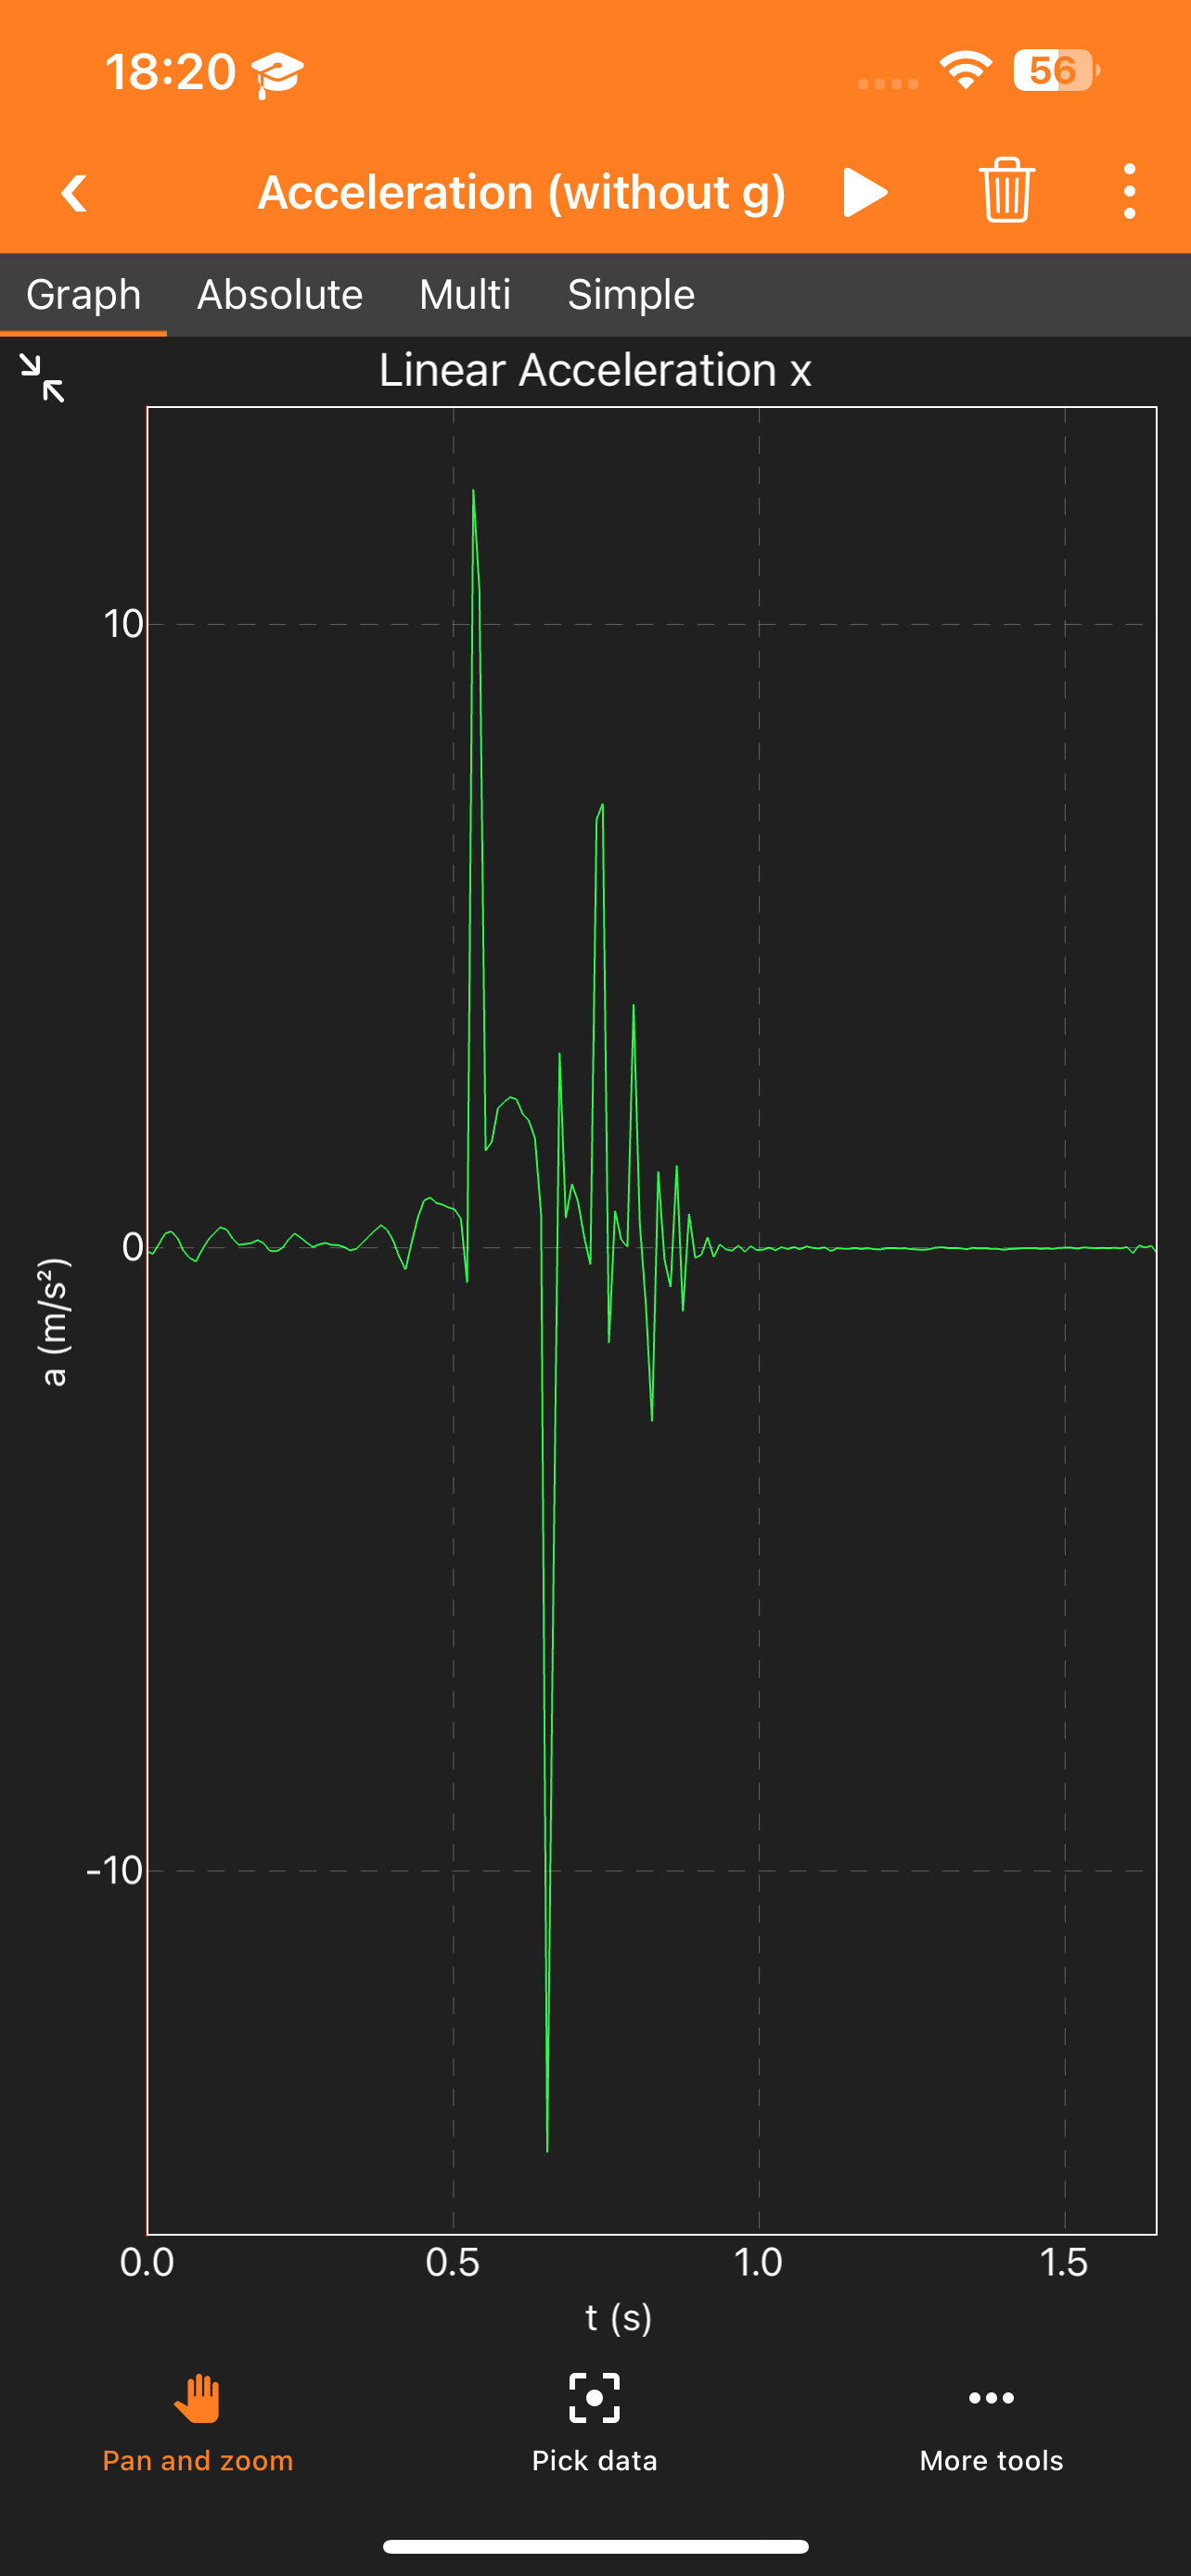
\includegraphics[width=.7\linewidth]{images/Lab.02/PhoneDropX.PNG}
\end{center}
\caption{Screenshot of enlarged x-axis plot.}
\label{fig:Lab02-PhoneDropX}
\end{figure}

\begin{figure}[H] % Example of including images
\begin{center}
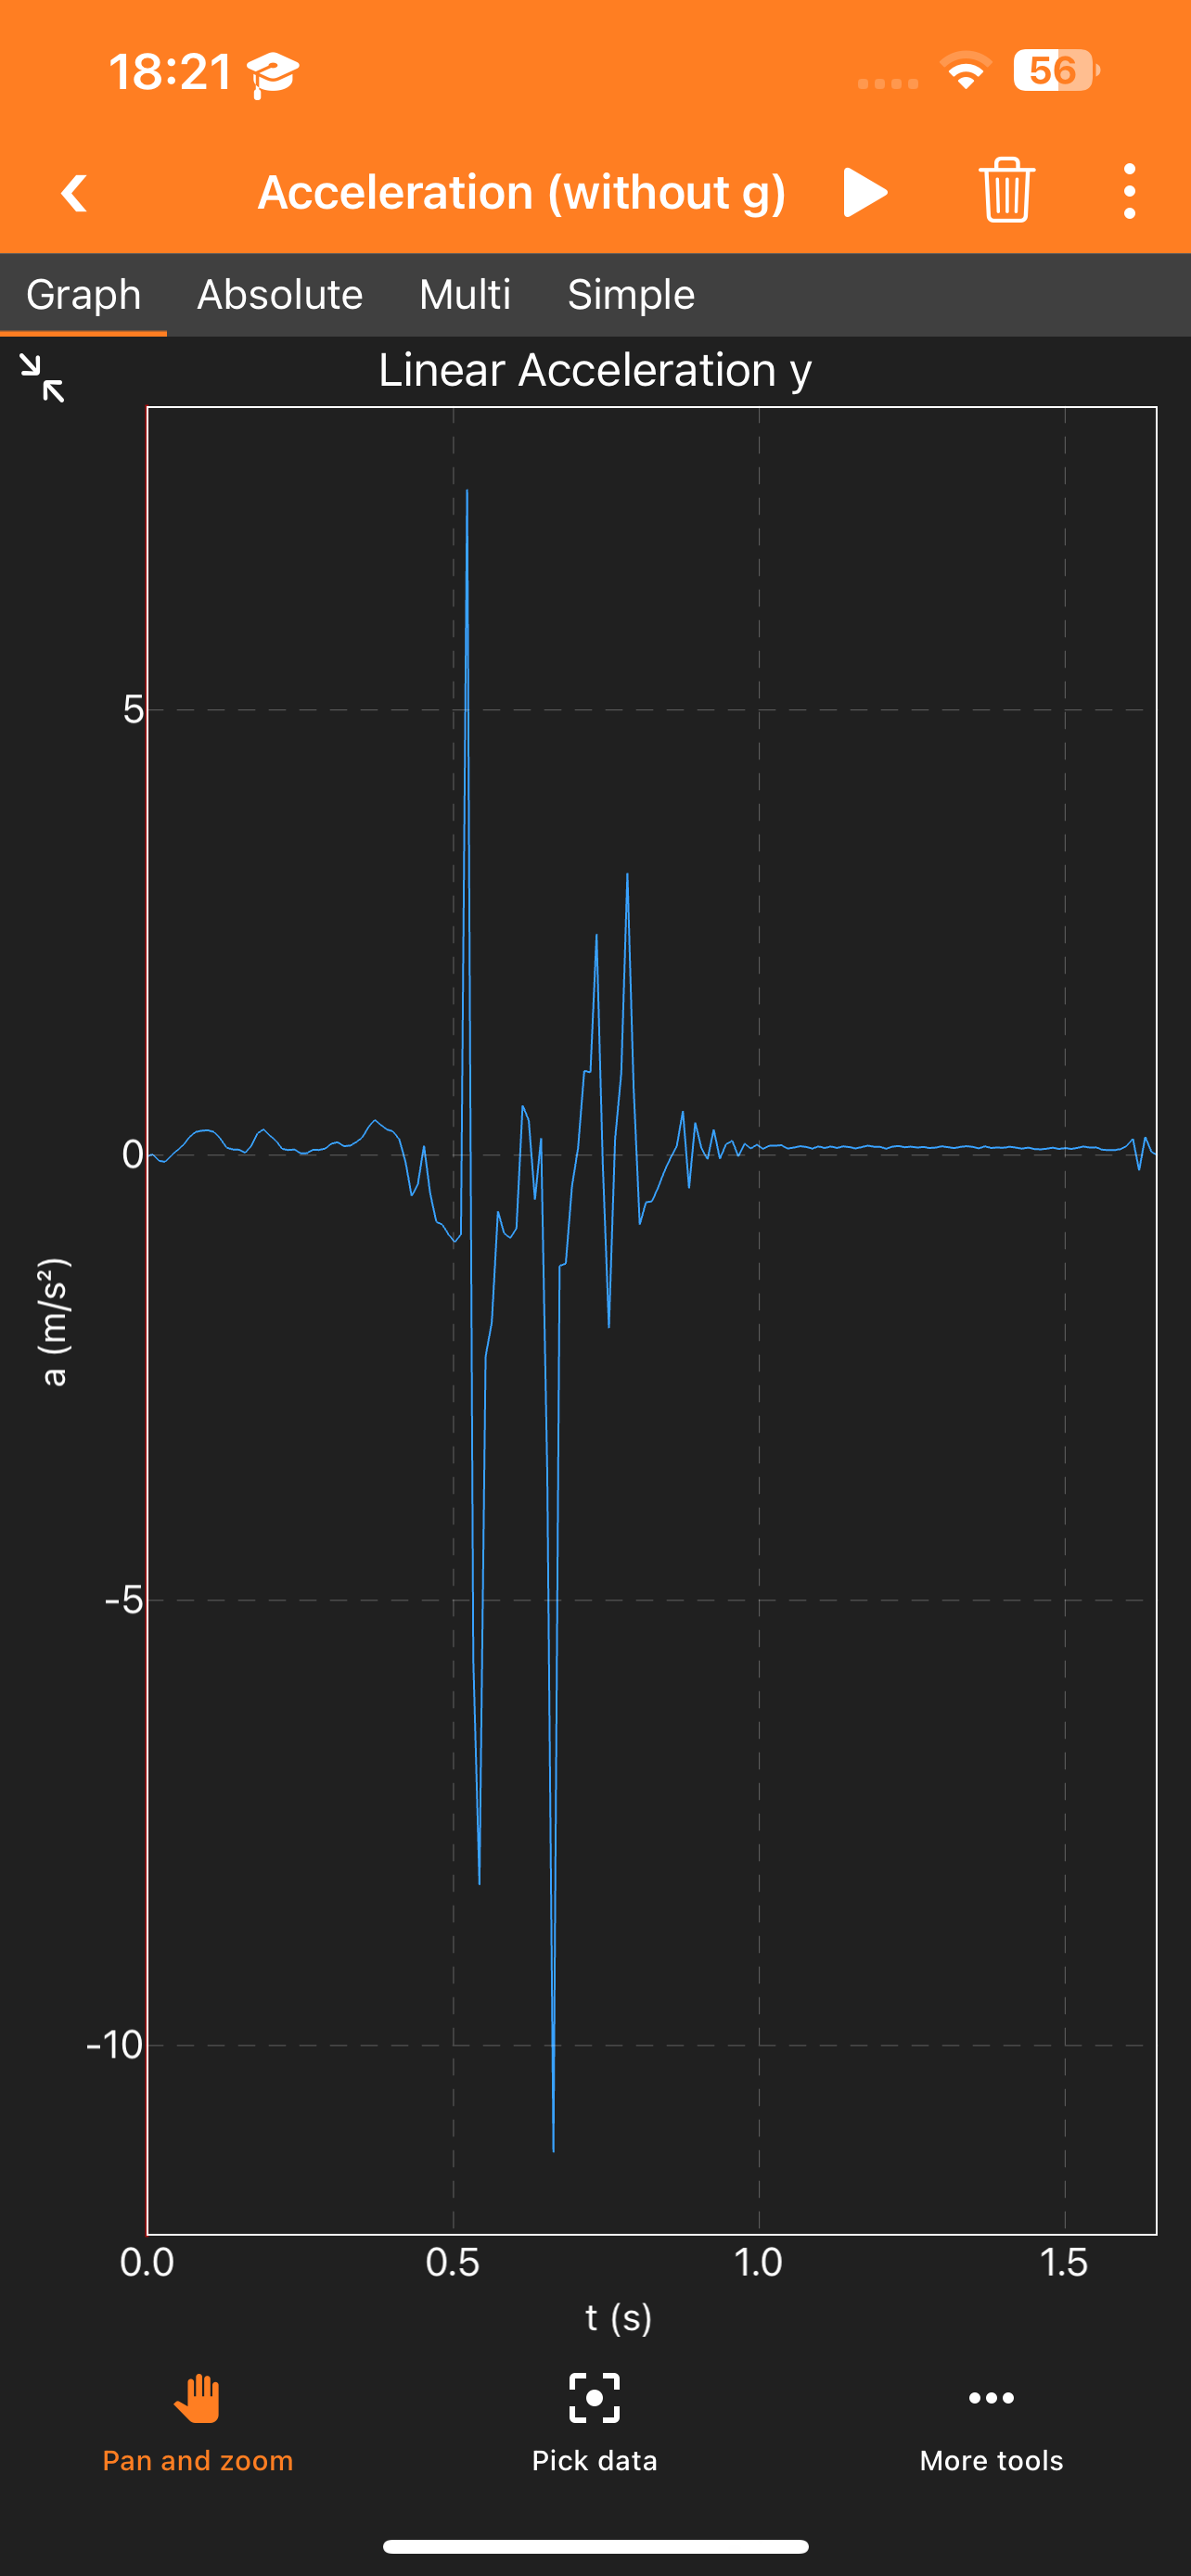
\includegraphics[width=.7\linewidth]{images/Lab.02/PhoneDropY.PNG}
\end{center}
\caption{Screenshot of enlarged y-axis plot.}
\label{fig:Lab02-PhoneDropY}
\end{figure}

\begin{figure}[H] % Example of including images
\begin{center}
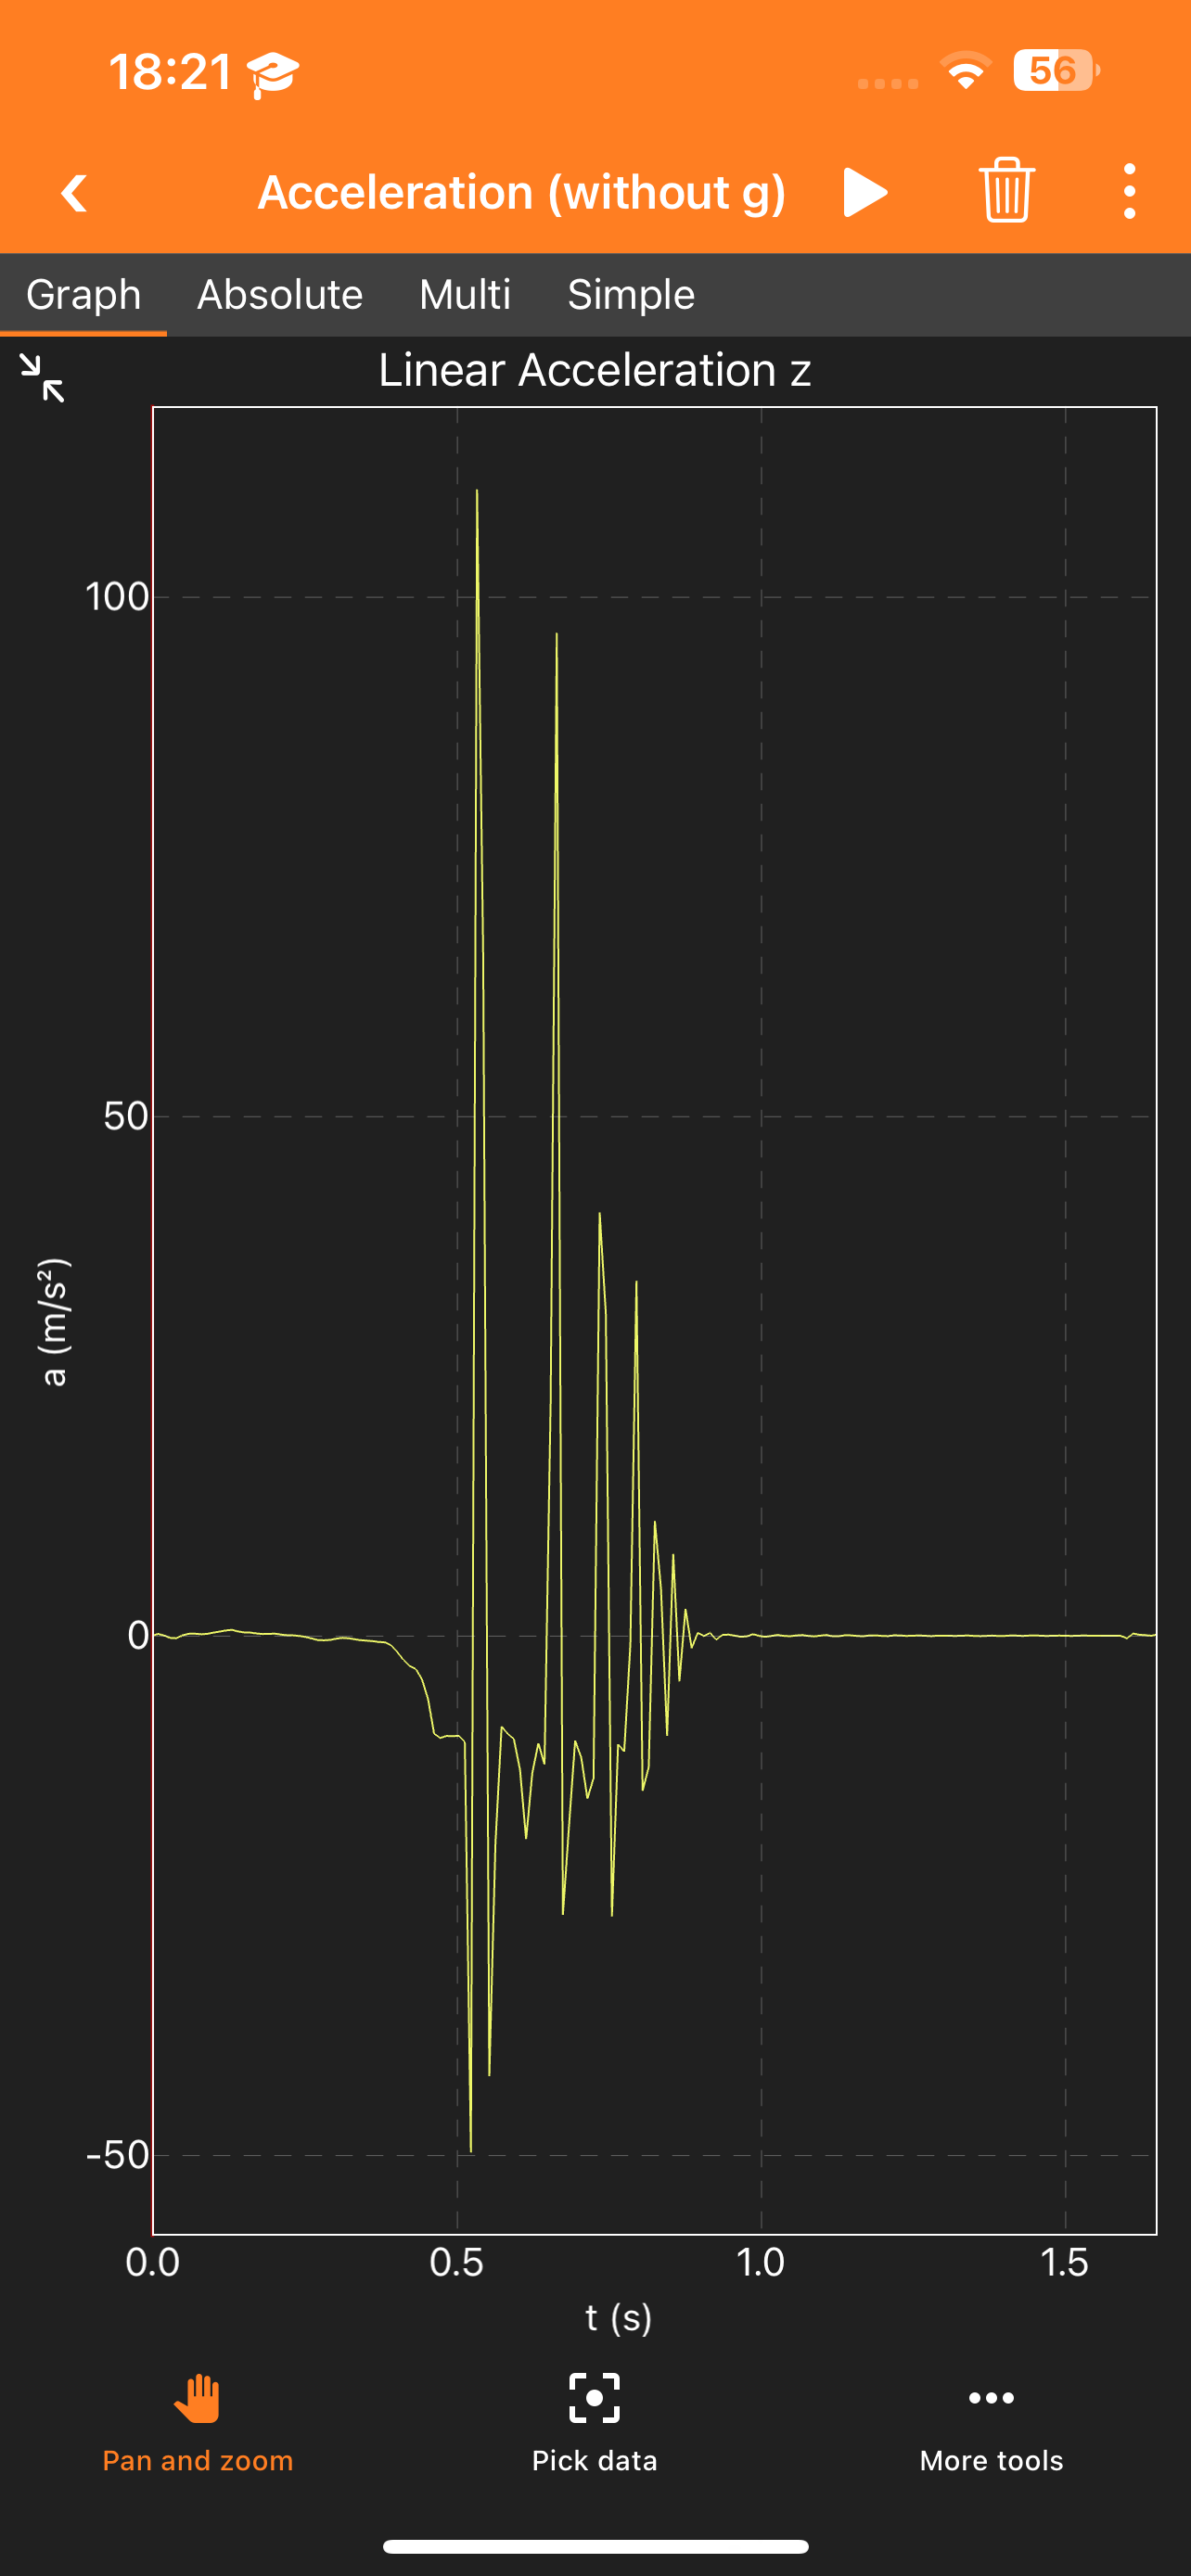
\includegraphics[width=.7\linewidth]{images/Lab.02/PhoneDropZ.PNG}
\end{center}
\caption{Screenshot of enlarged z-axis plot.}
\label{fig:Lab02-PhoneDropZ}
\end{figure}

\begin{figure}[H] % Example of including images
\begin{center}
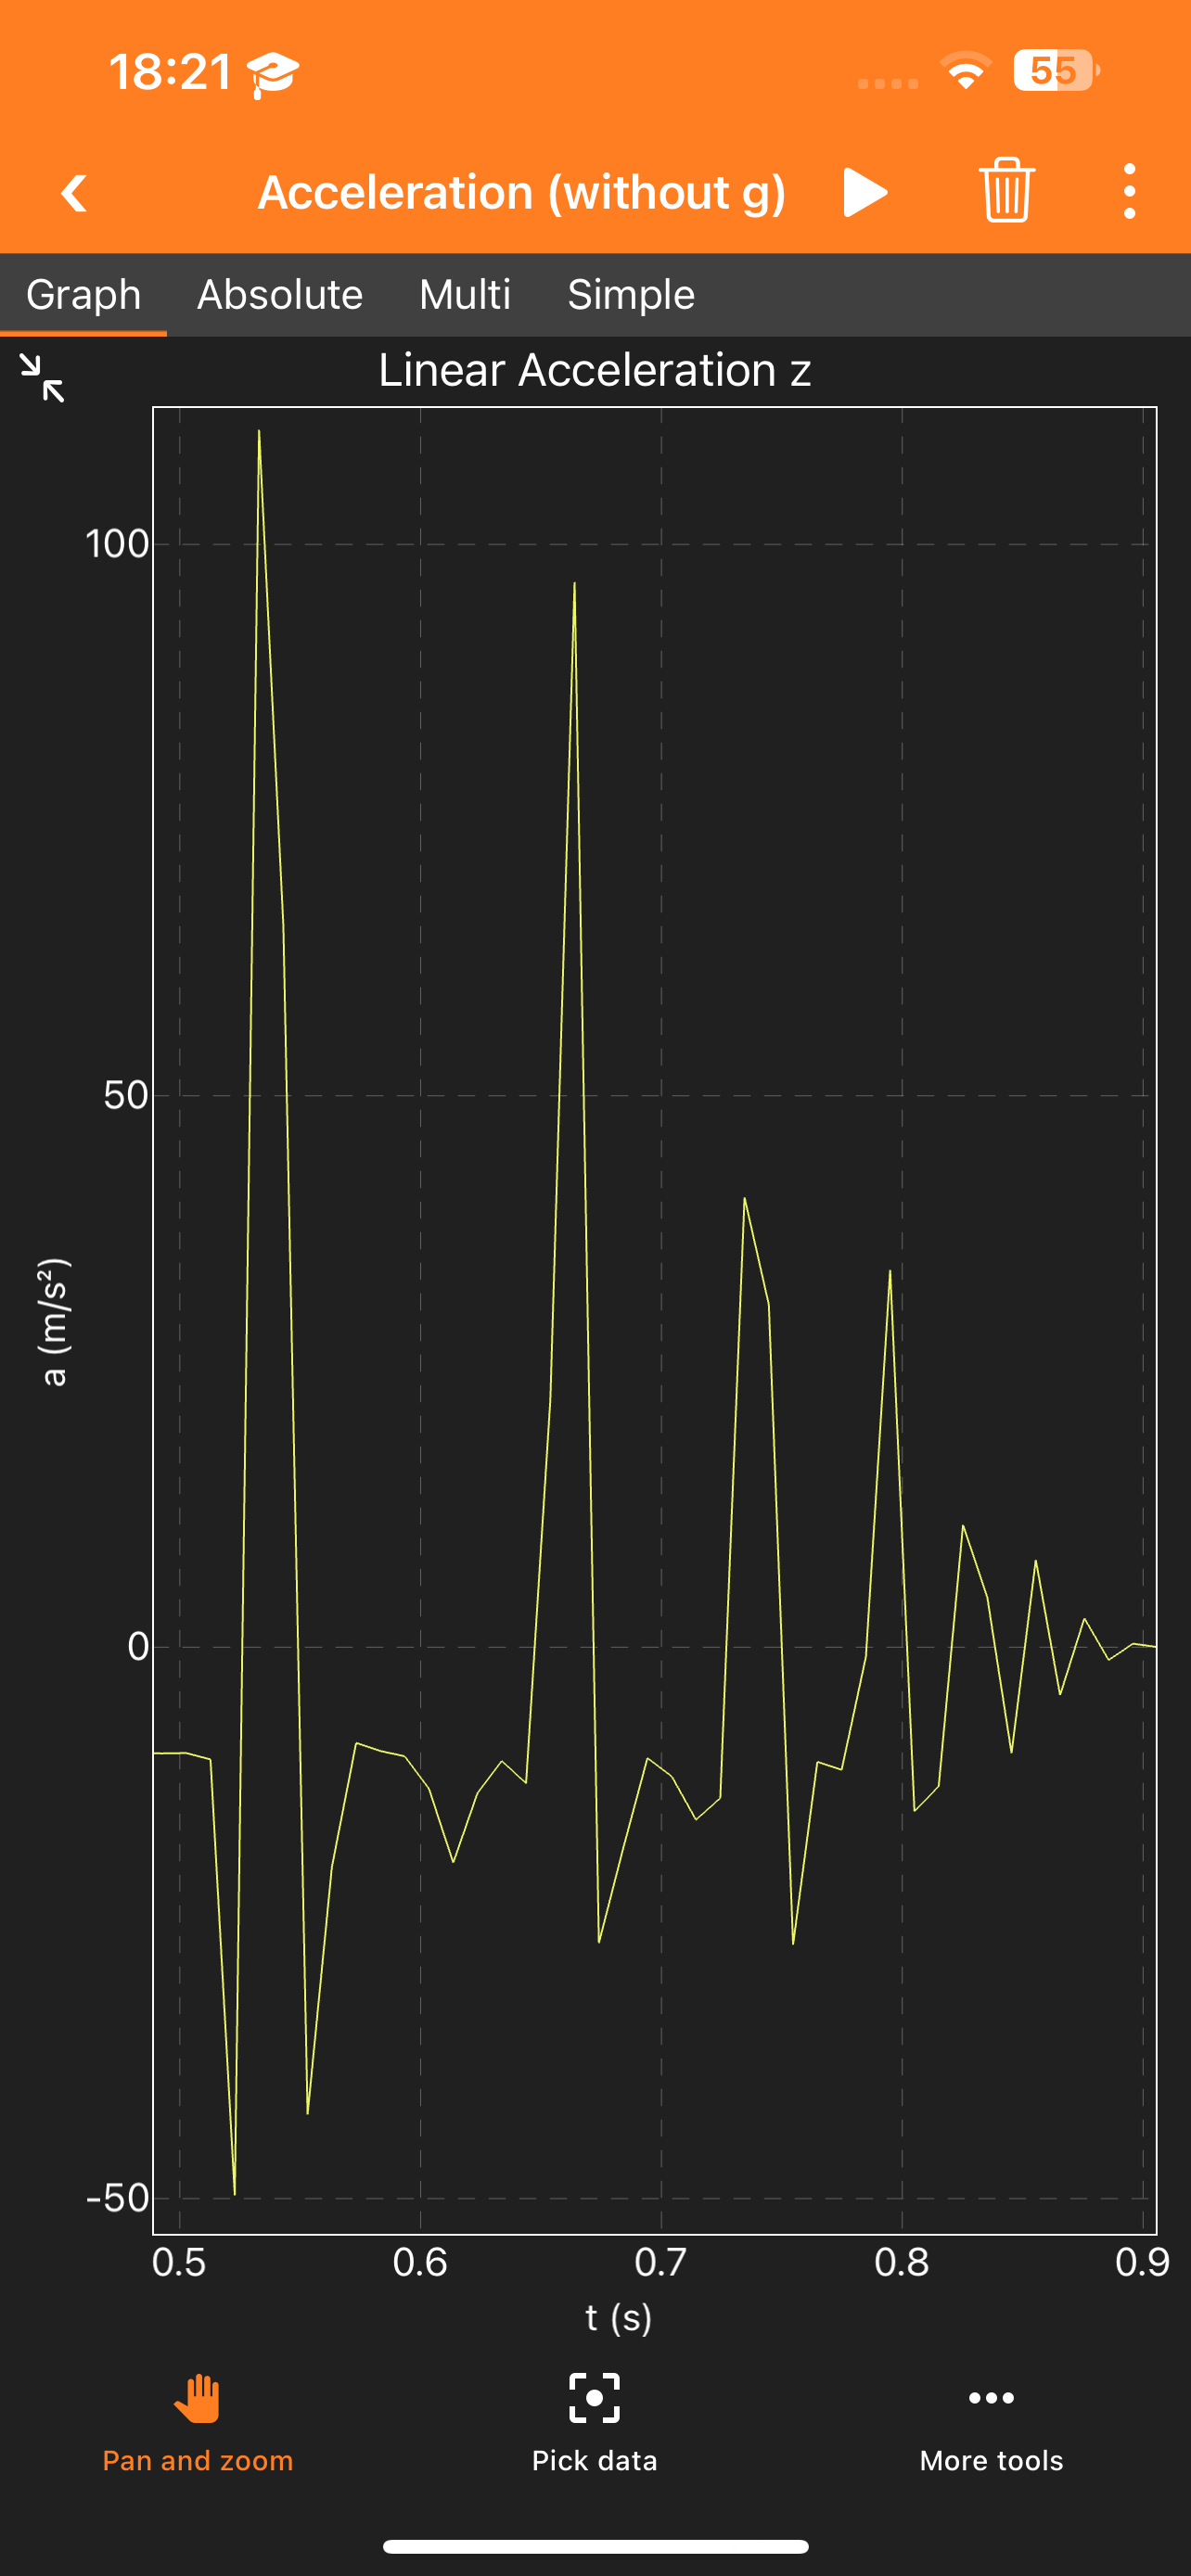
\includegraphics[width=.7\linewidth]{images/Lab.02/PhoneDropZzoomed.PNG}
\end{center}
\caption{Screenshot of zoomed-in z-axis plot}
\label{fig:Lab02-PhoneDropZzoomed}
\end{figure}

\begin{figure}[H] % Example of including images
\begin{center}
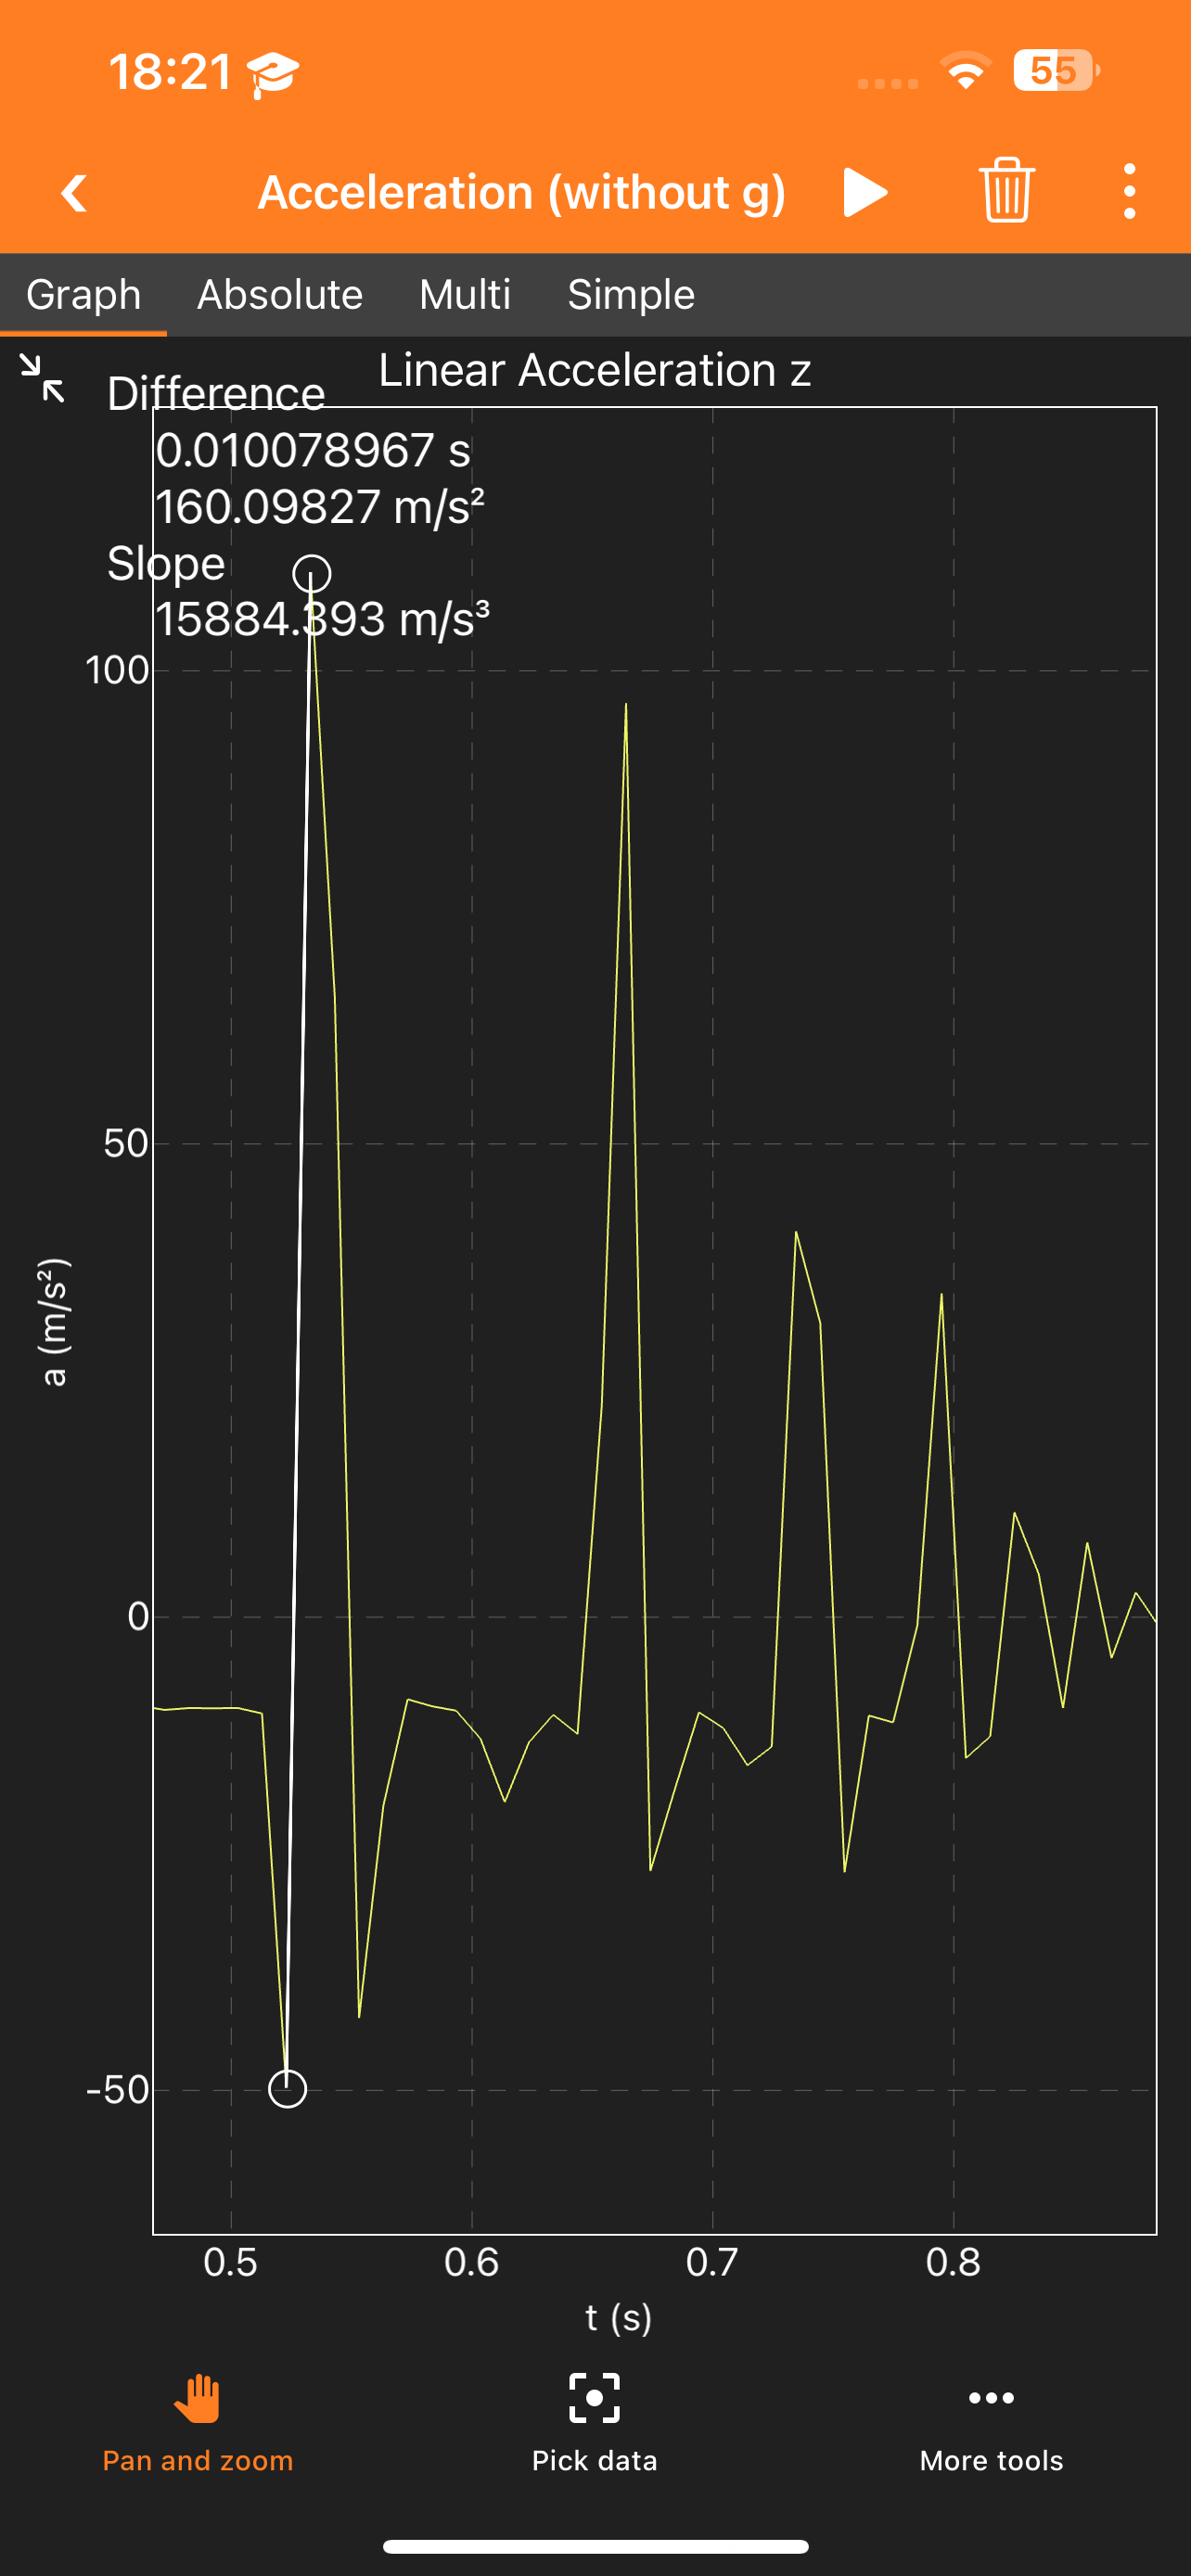
\includegraphics[width=.7\linewidth]{images/Lab.02/PhoneDropZAnnotated1.PNG}
\end{center}
\caption{First screenshot of z-axis plot with data points}
\label{fig:Lab02-PhoneDropZAnnotated1}
\end{figure}

\begin{figure}[H] % Example of including images
\begin{center}
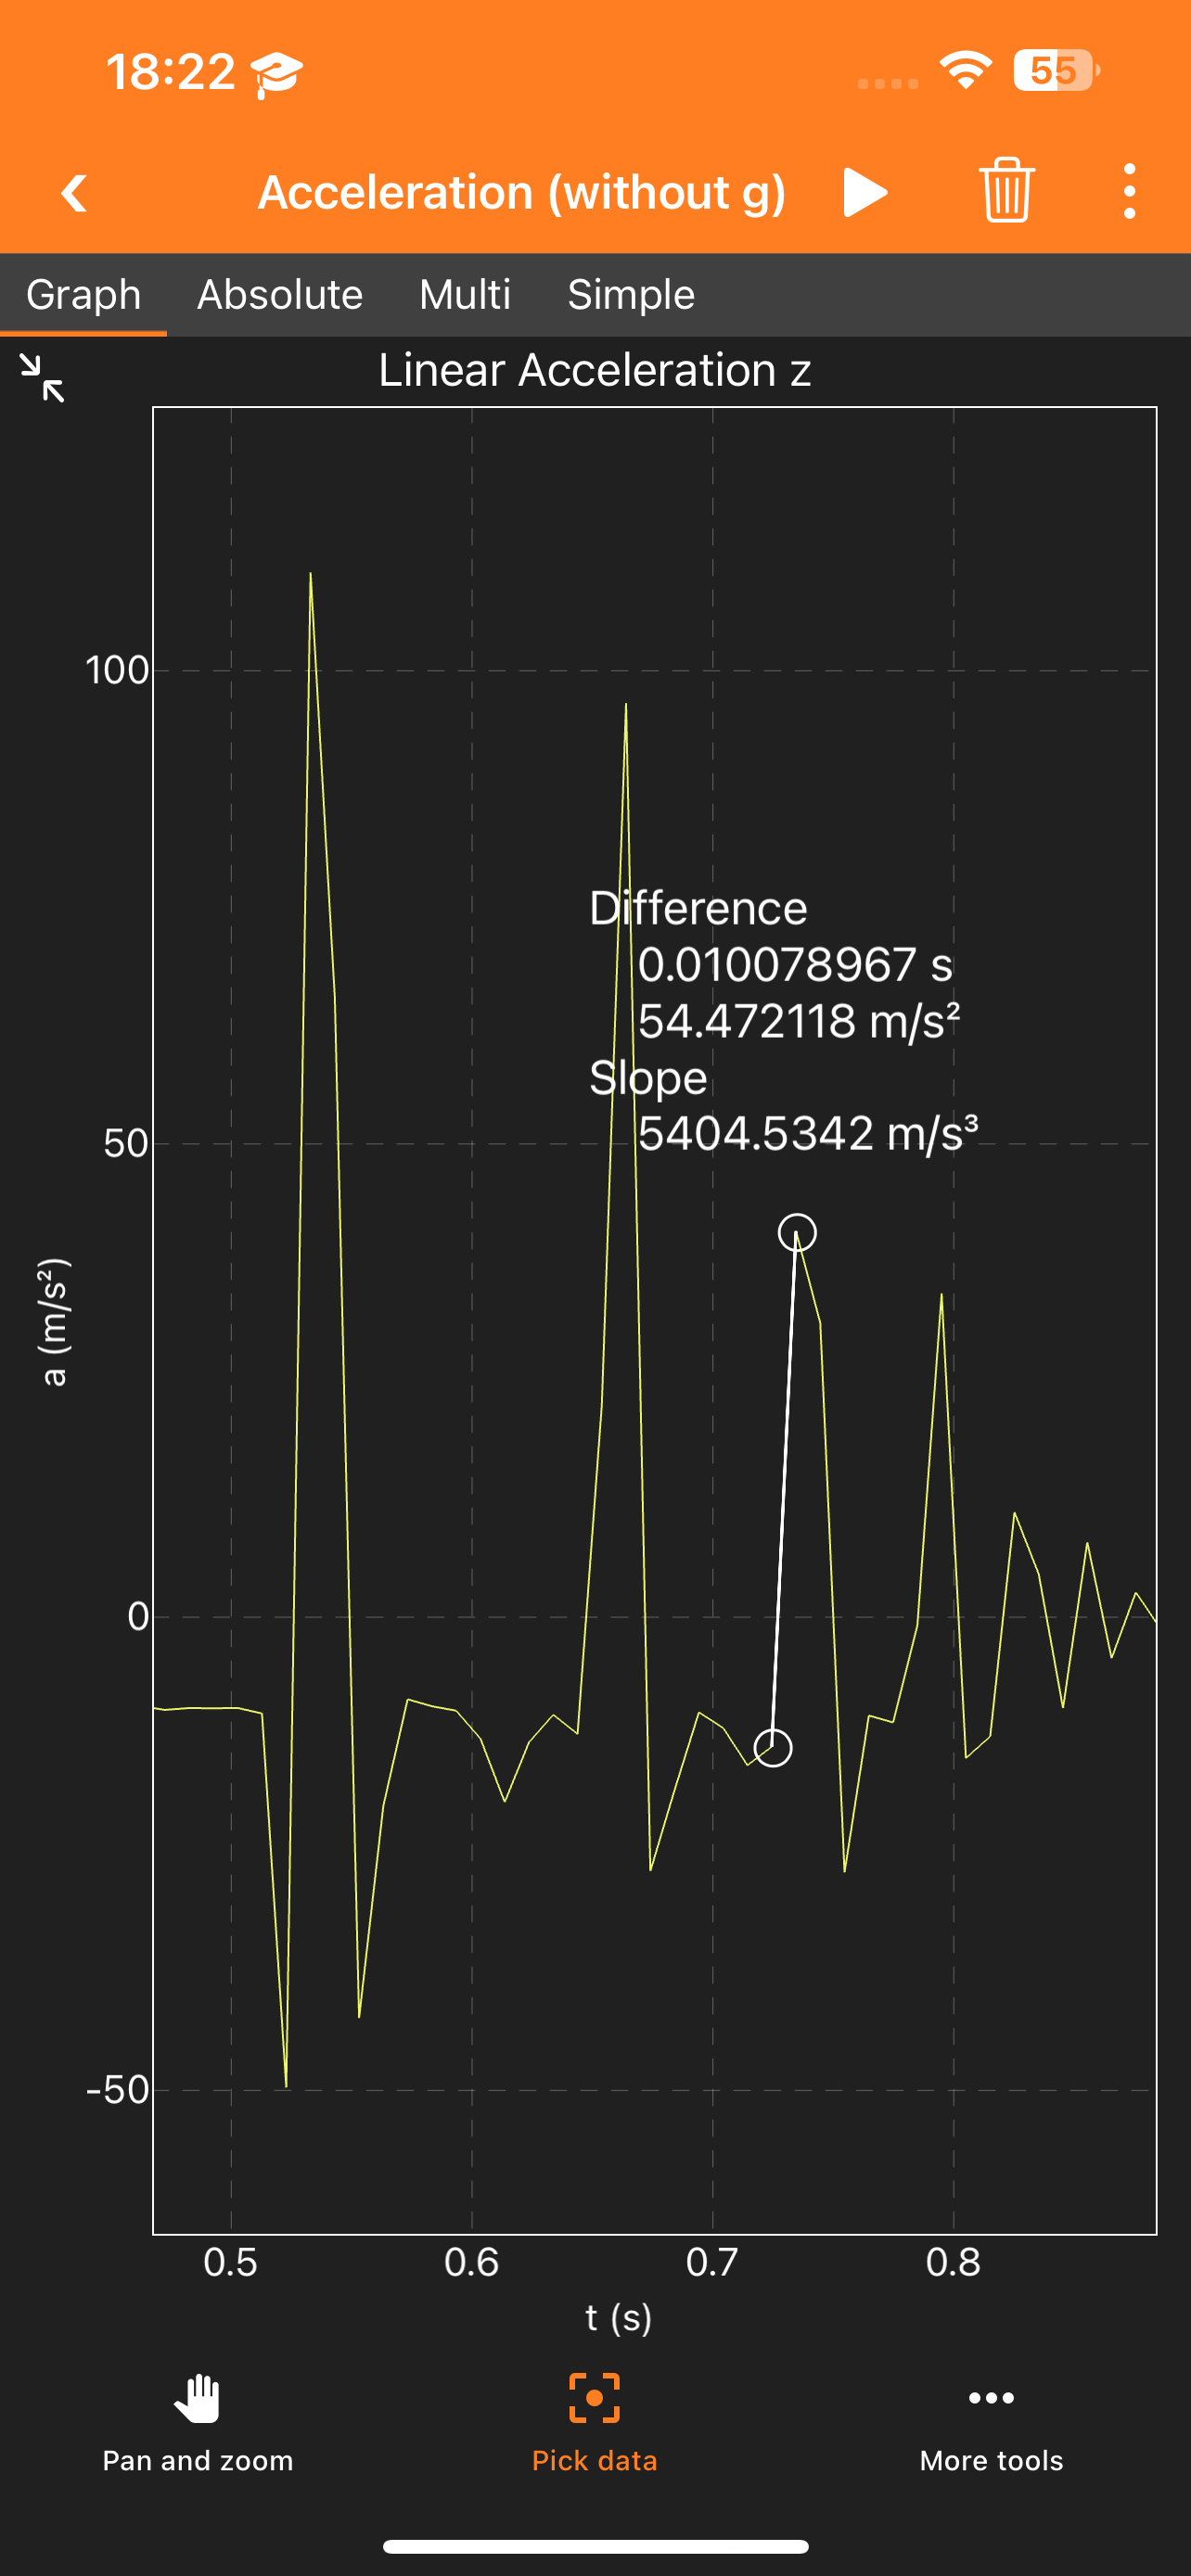
\includegraphics[width=.7\linewidth]{images/Lab.02/PhoneDropZAnnotated2.PNG}
\end{center}
\caption{Second screenshot of z-axis plot with data points}
\label{fig:Lab02-PhoneDropZAnnotated2}
\end{figure}

\begin{figure}[H] % Example of including images
\begin{center}
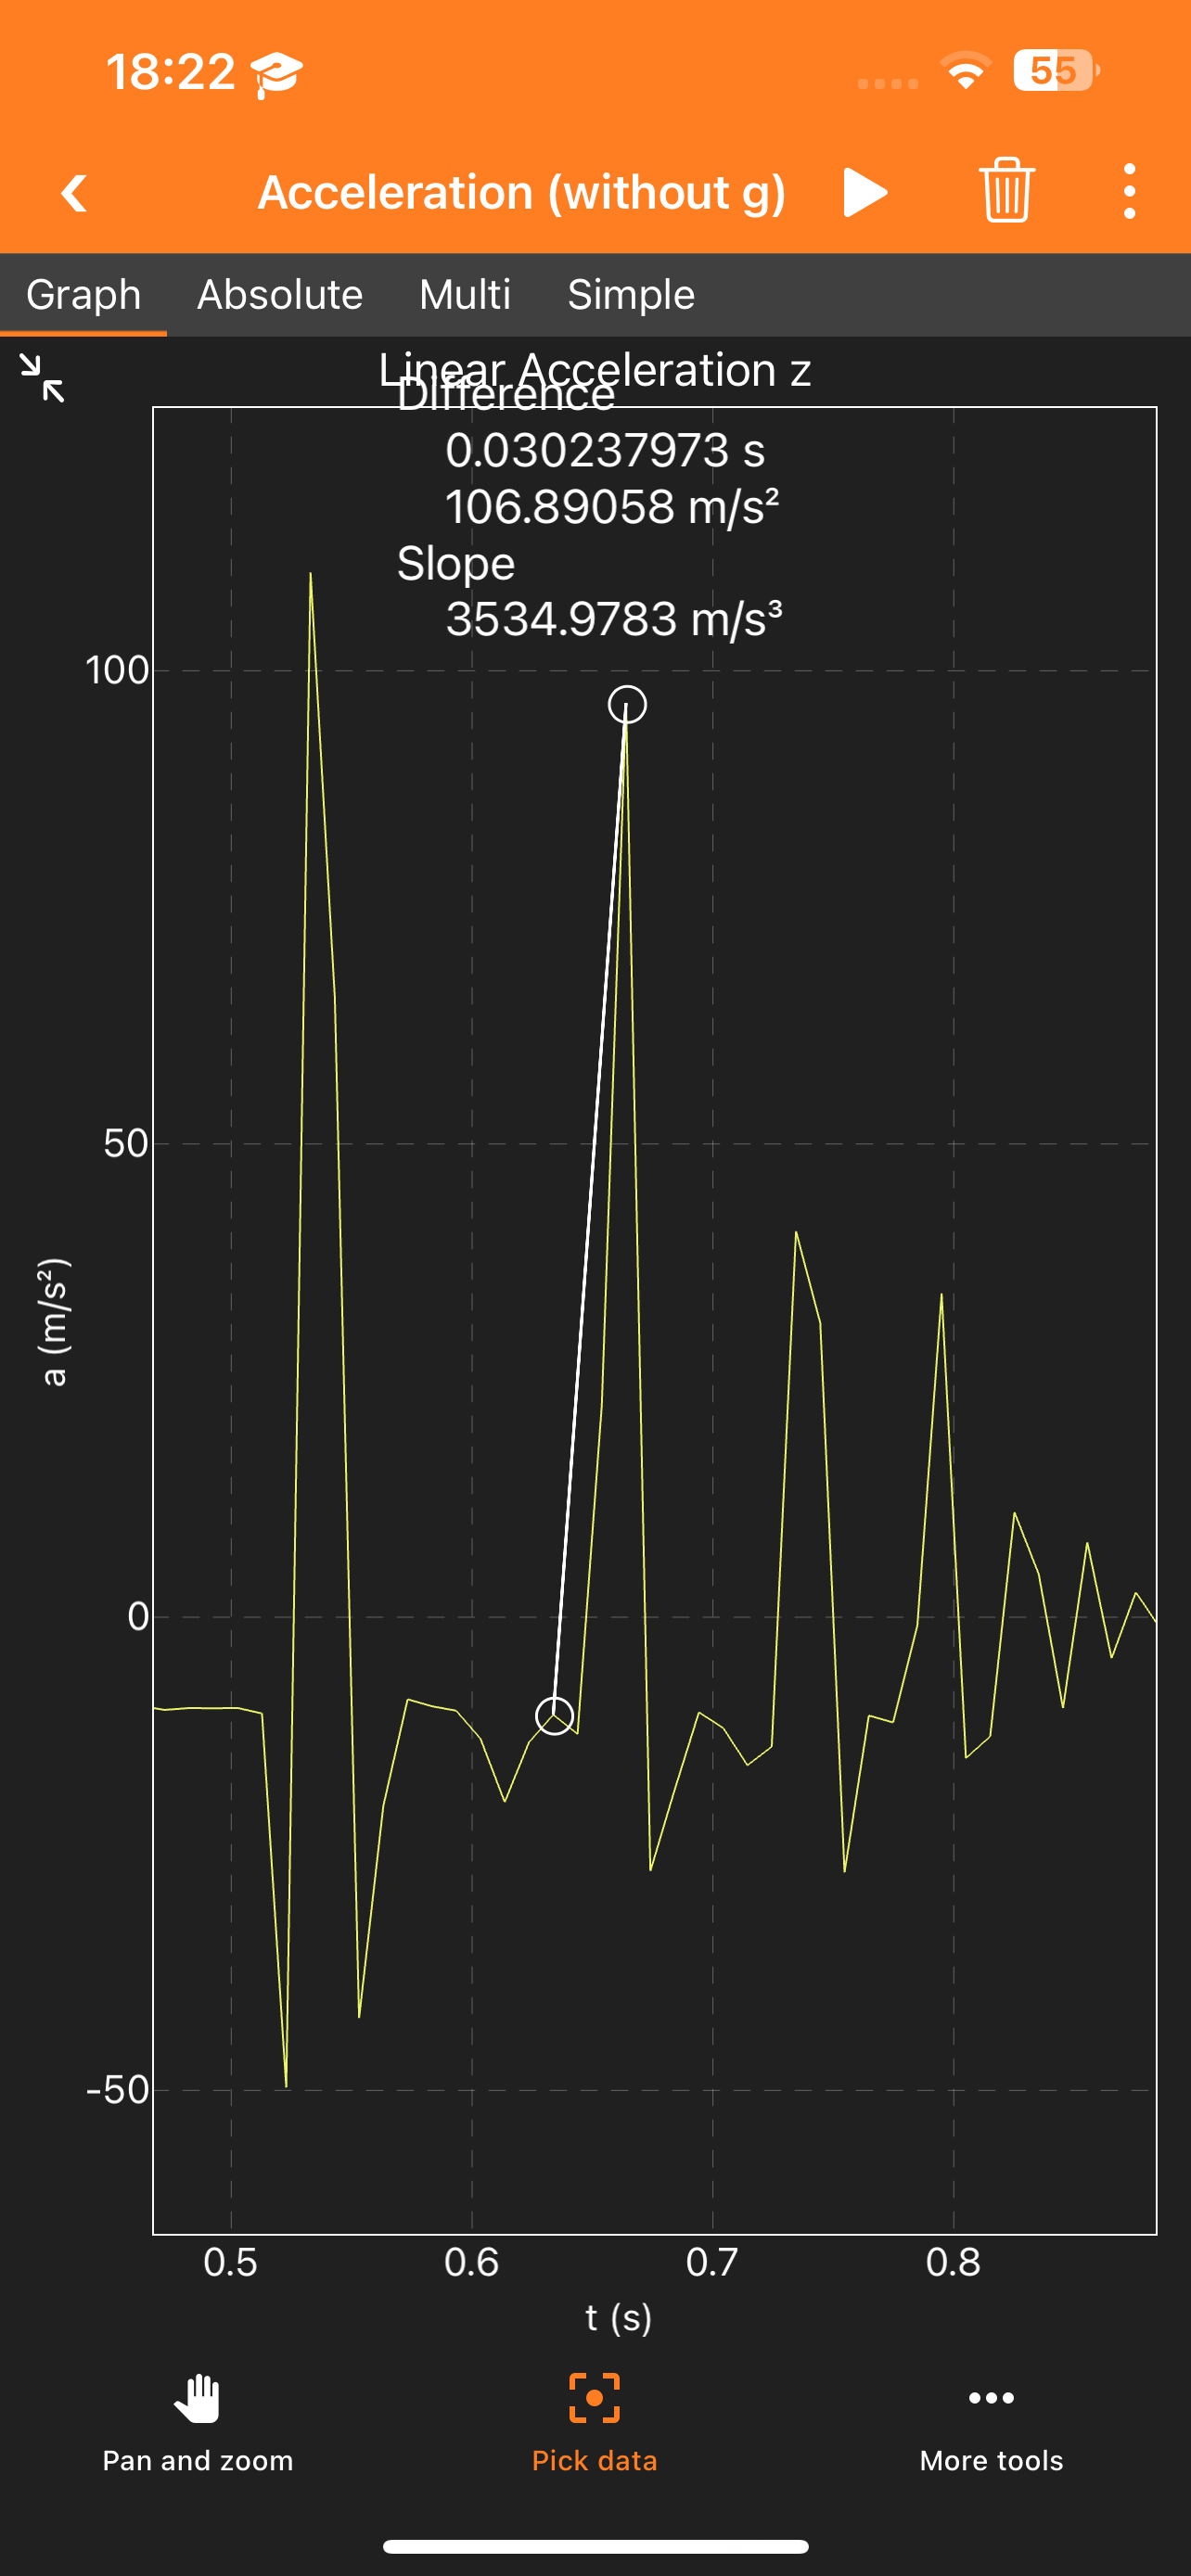
\includegraphics[width=.7\linewidth]{images/Lab.02/PhoneDropZAnnotated3.PNG}
\end{center}
\caption{Third screenshot of z-axis plot with data points}
\label{fig:Lab02-PhoneDropZAnnotated3}
\end{figure}

\begin{figure}[H] % Example of including images
\begin{center}
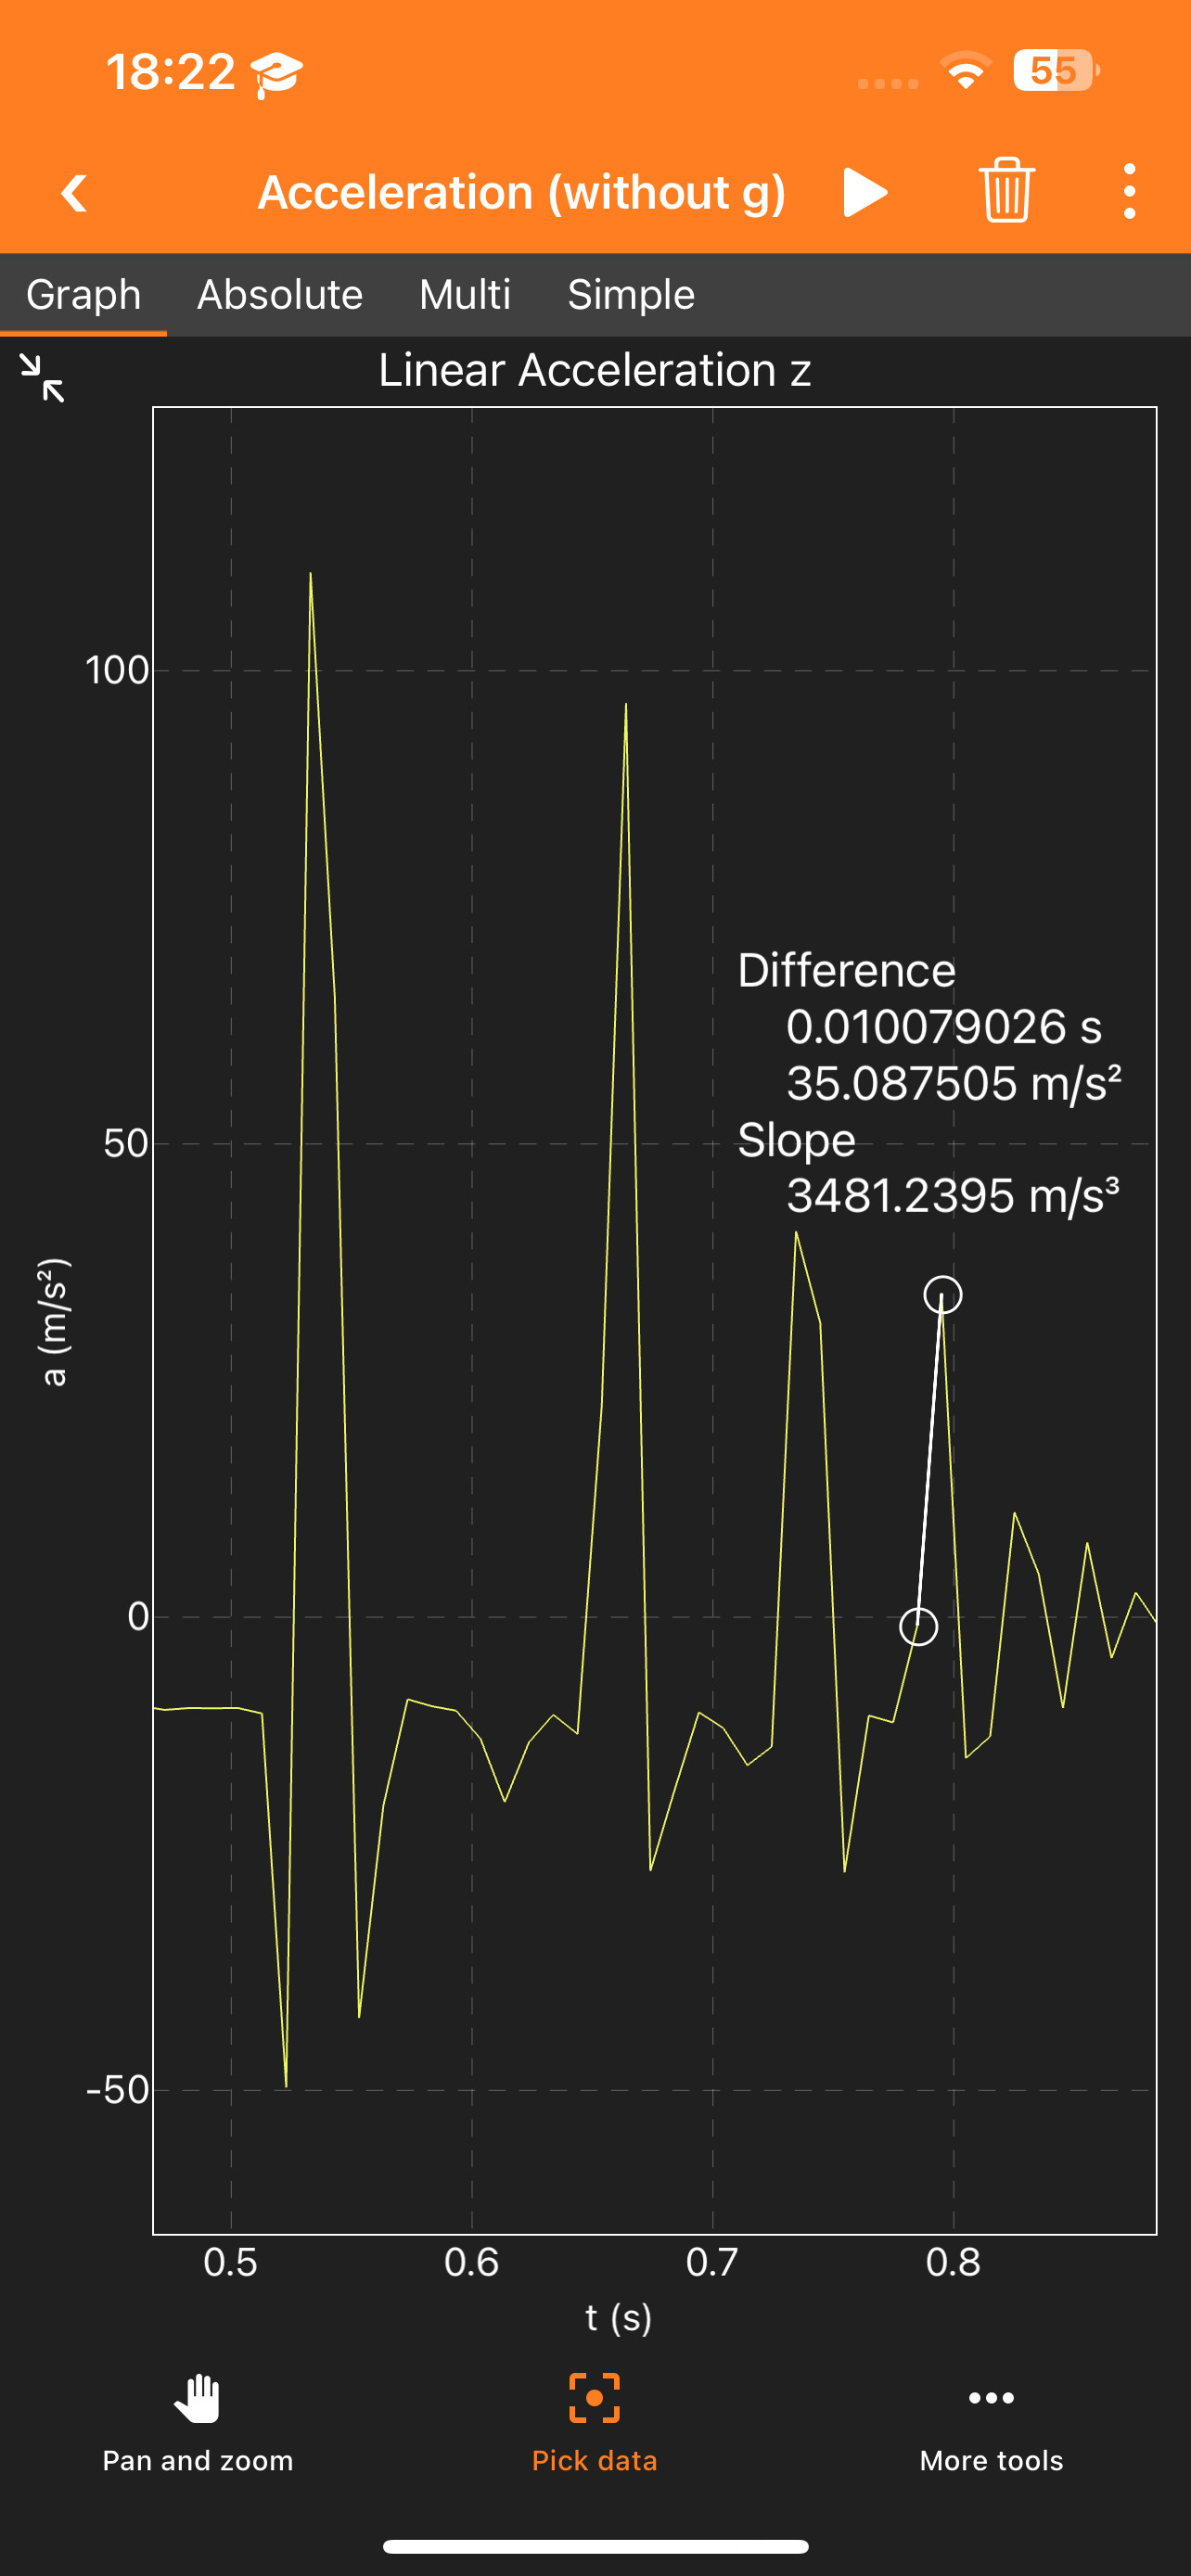
\includegraphics[width=.7\linewidth]{images/Lab.02/PhoneDropZAnnotated4.PNG}
\end{center}
\caption{Fourth screenshot of z-axis plot with data points}
\label{fig:Lab02-PhoneDropZAnnotated4}
\end{figure}

\begin{figure}[H] % Example of including images
\begin{center}
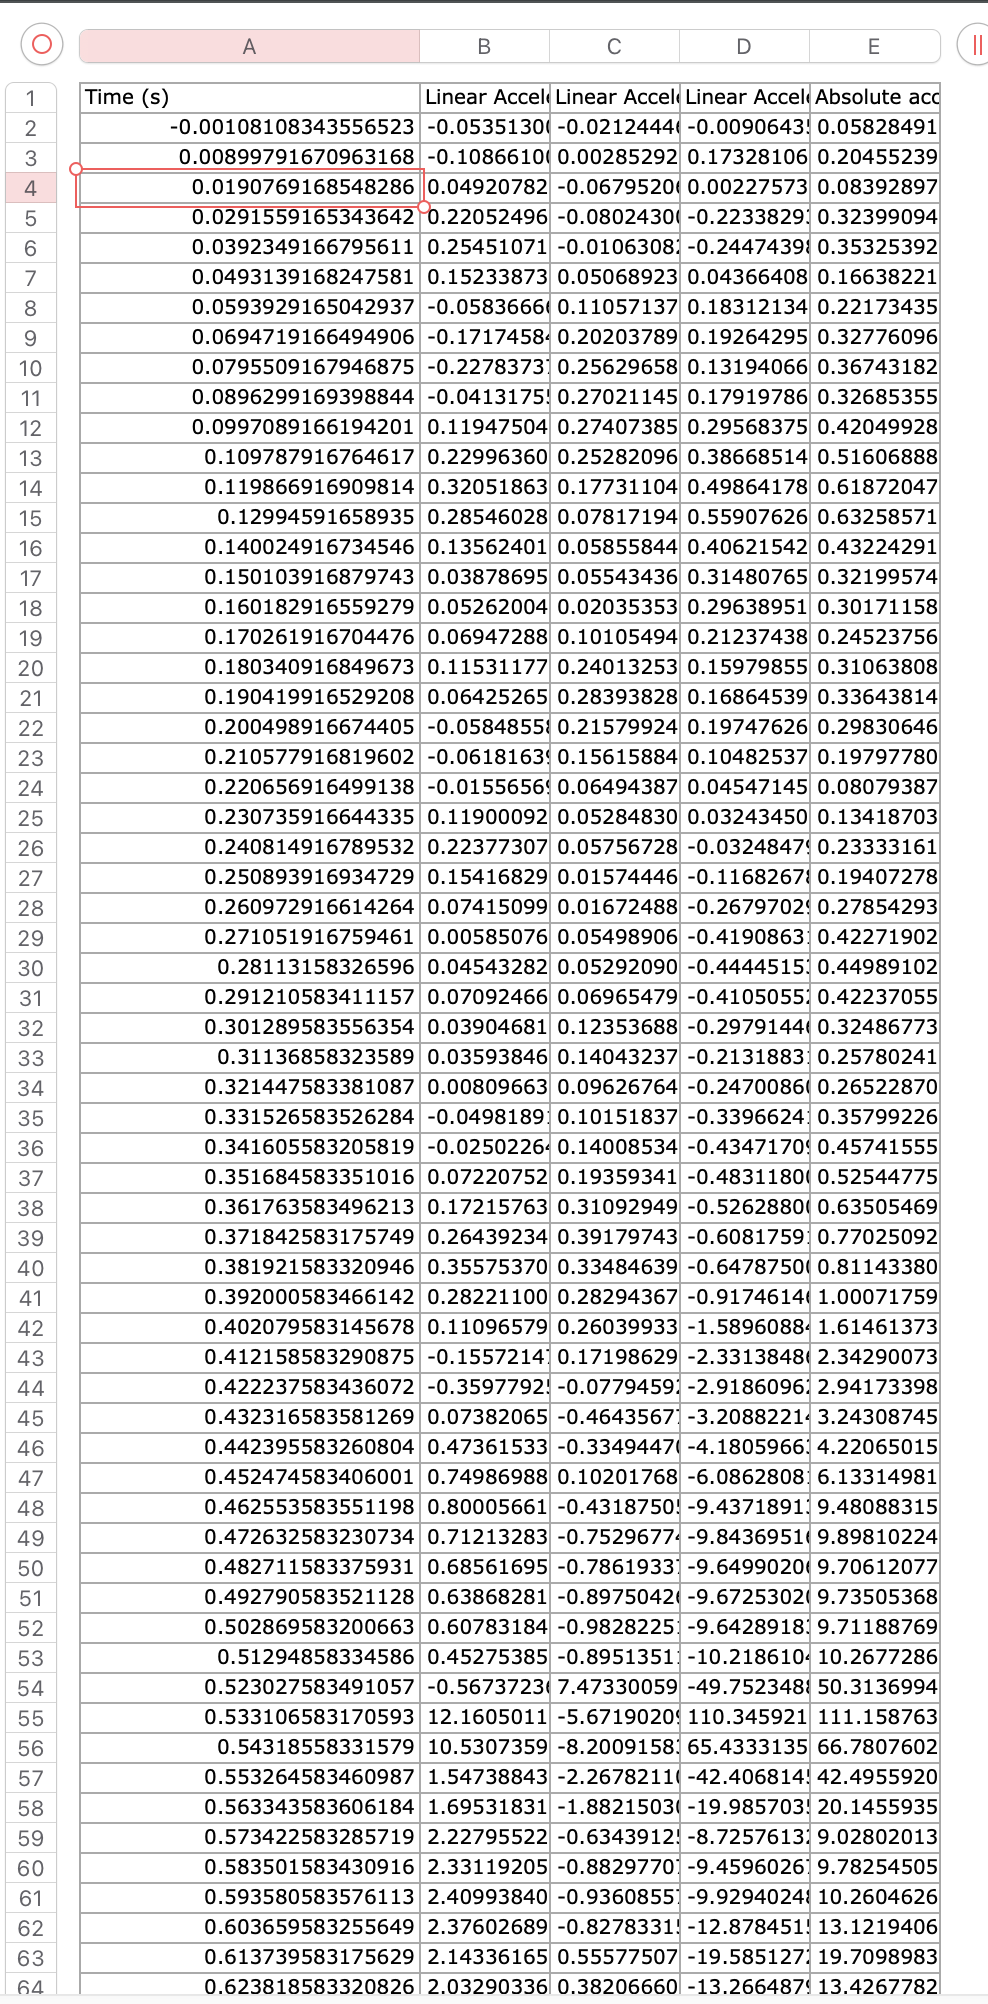
\includegraphics[width=.7\linewidth]{images/Lab.02/PhoneDropDataSet.png}
\end{center}
\caption{Screenshot of exported data from Phyphox}
\label{fig:Lab02-PhoneDropDataSet}
\end{figure}

\begin{figure}[H] % Example of including images
\begin{center}
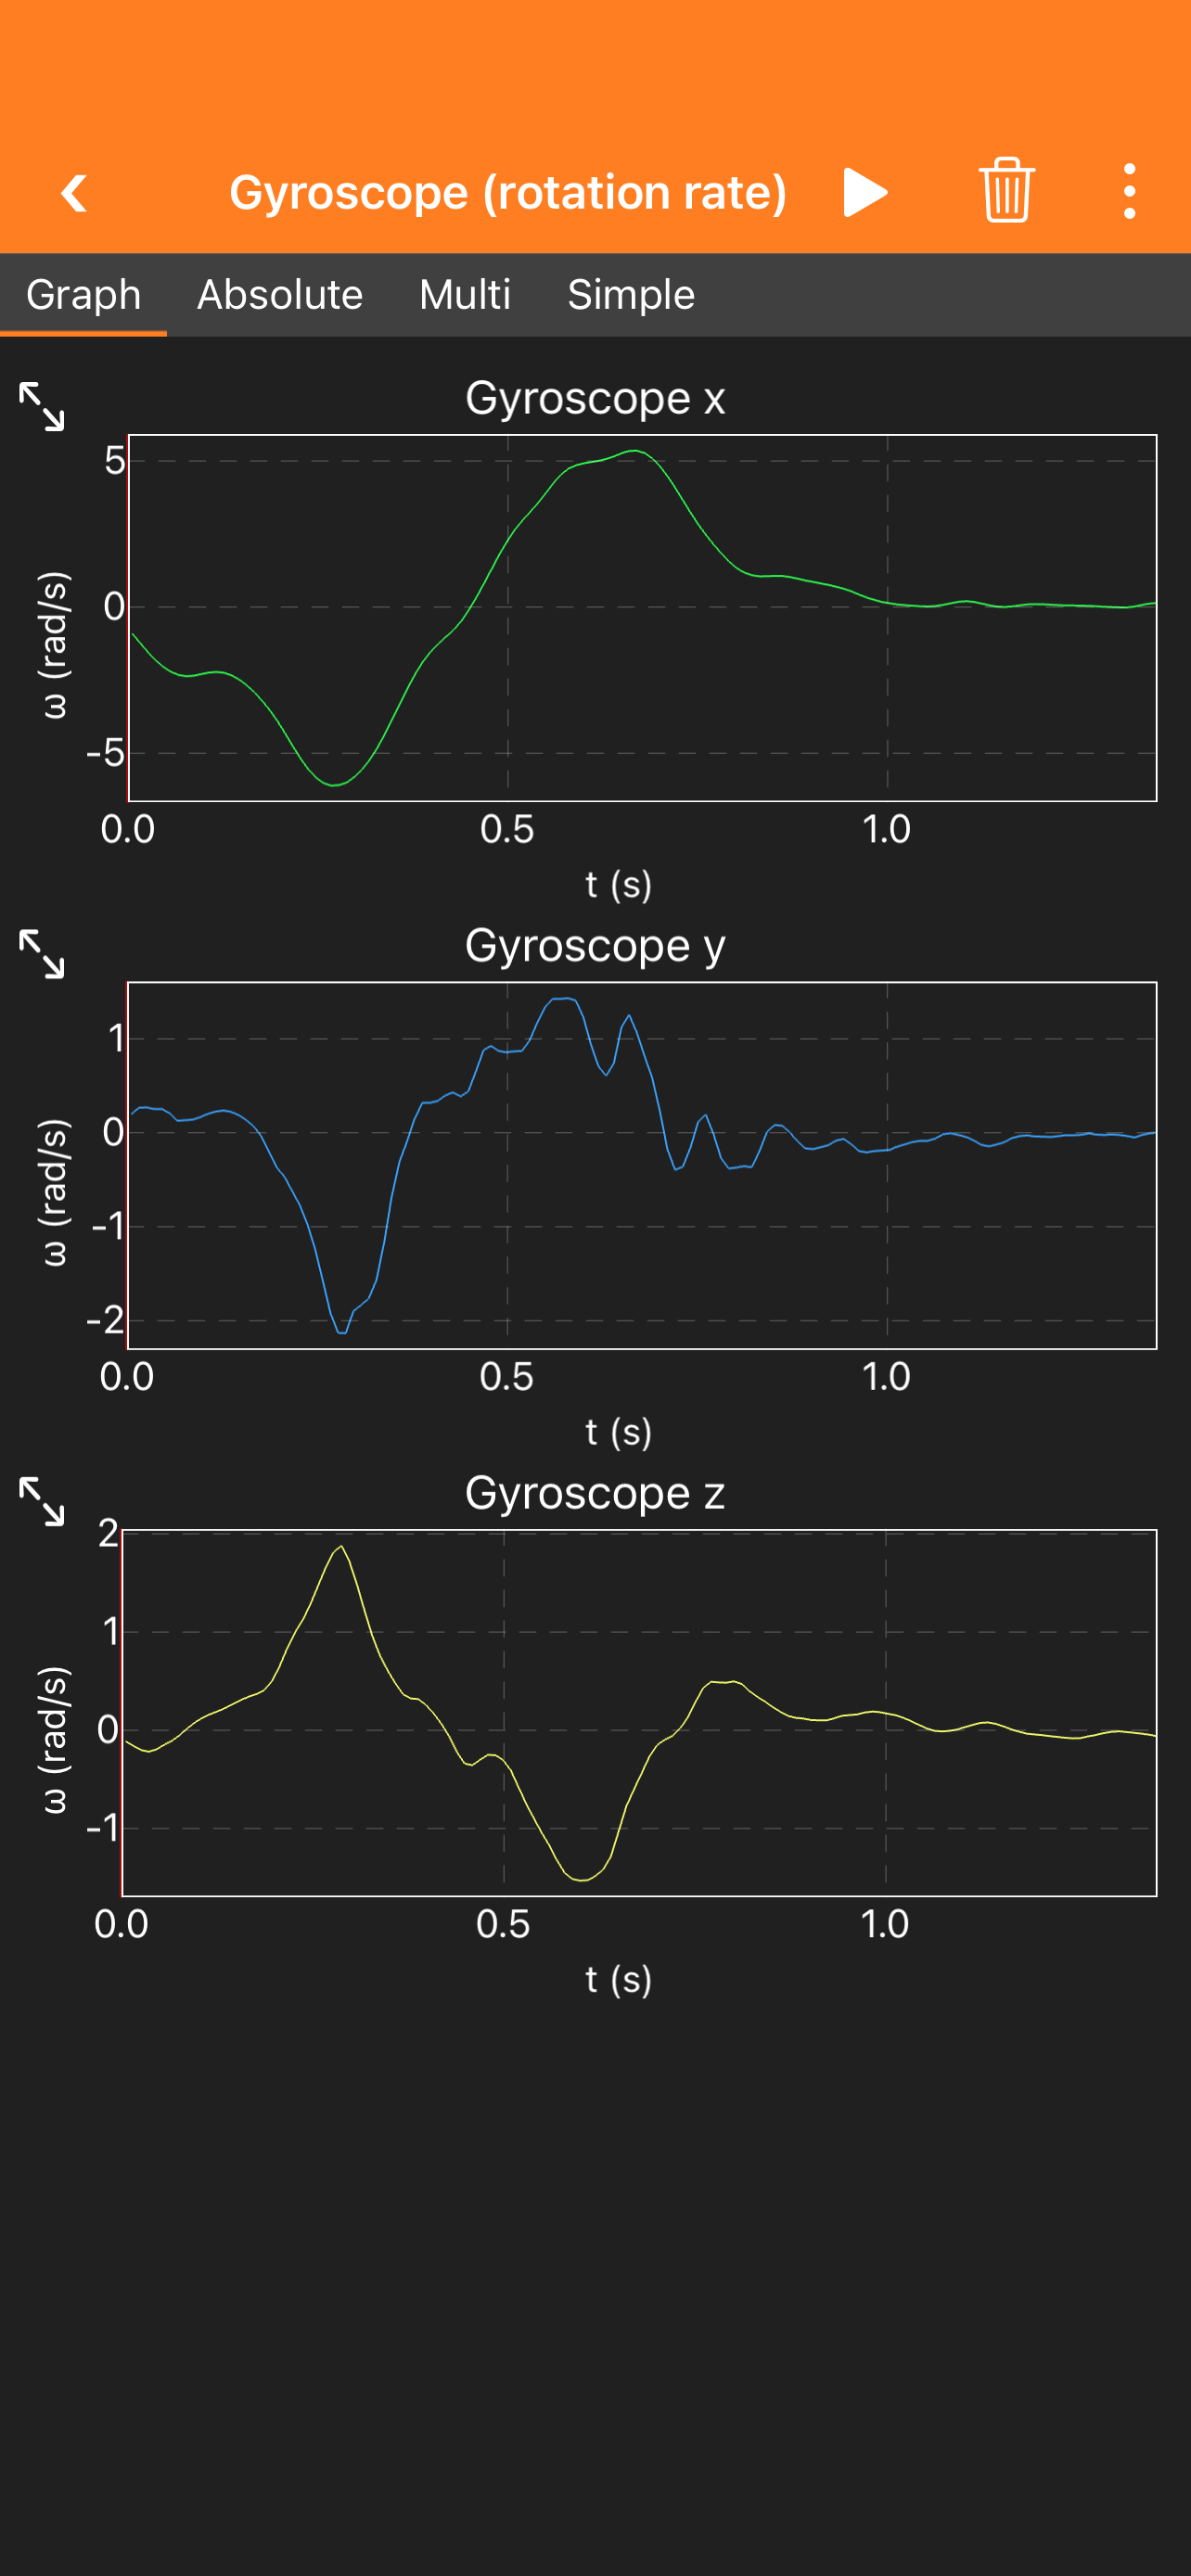
\includegraphics[width=.7\linewidth]{images/Lab.02/GyyroscopeX.PNG}
\end{center}
\caption{Screenshot of getting the Gyroscope data for the x-axis for the phone.}
\label{fig:Lab02-GyroscopeX}
\end{figure}

\begin{figure}[H] % Example of including images
\begin{center}
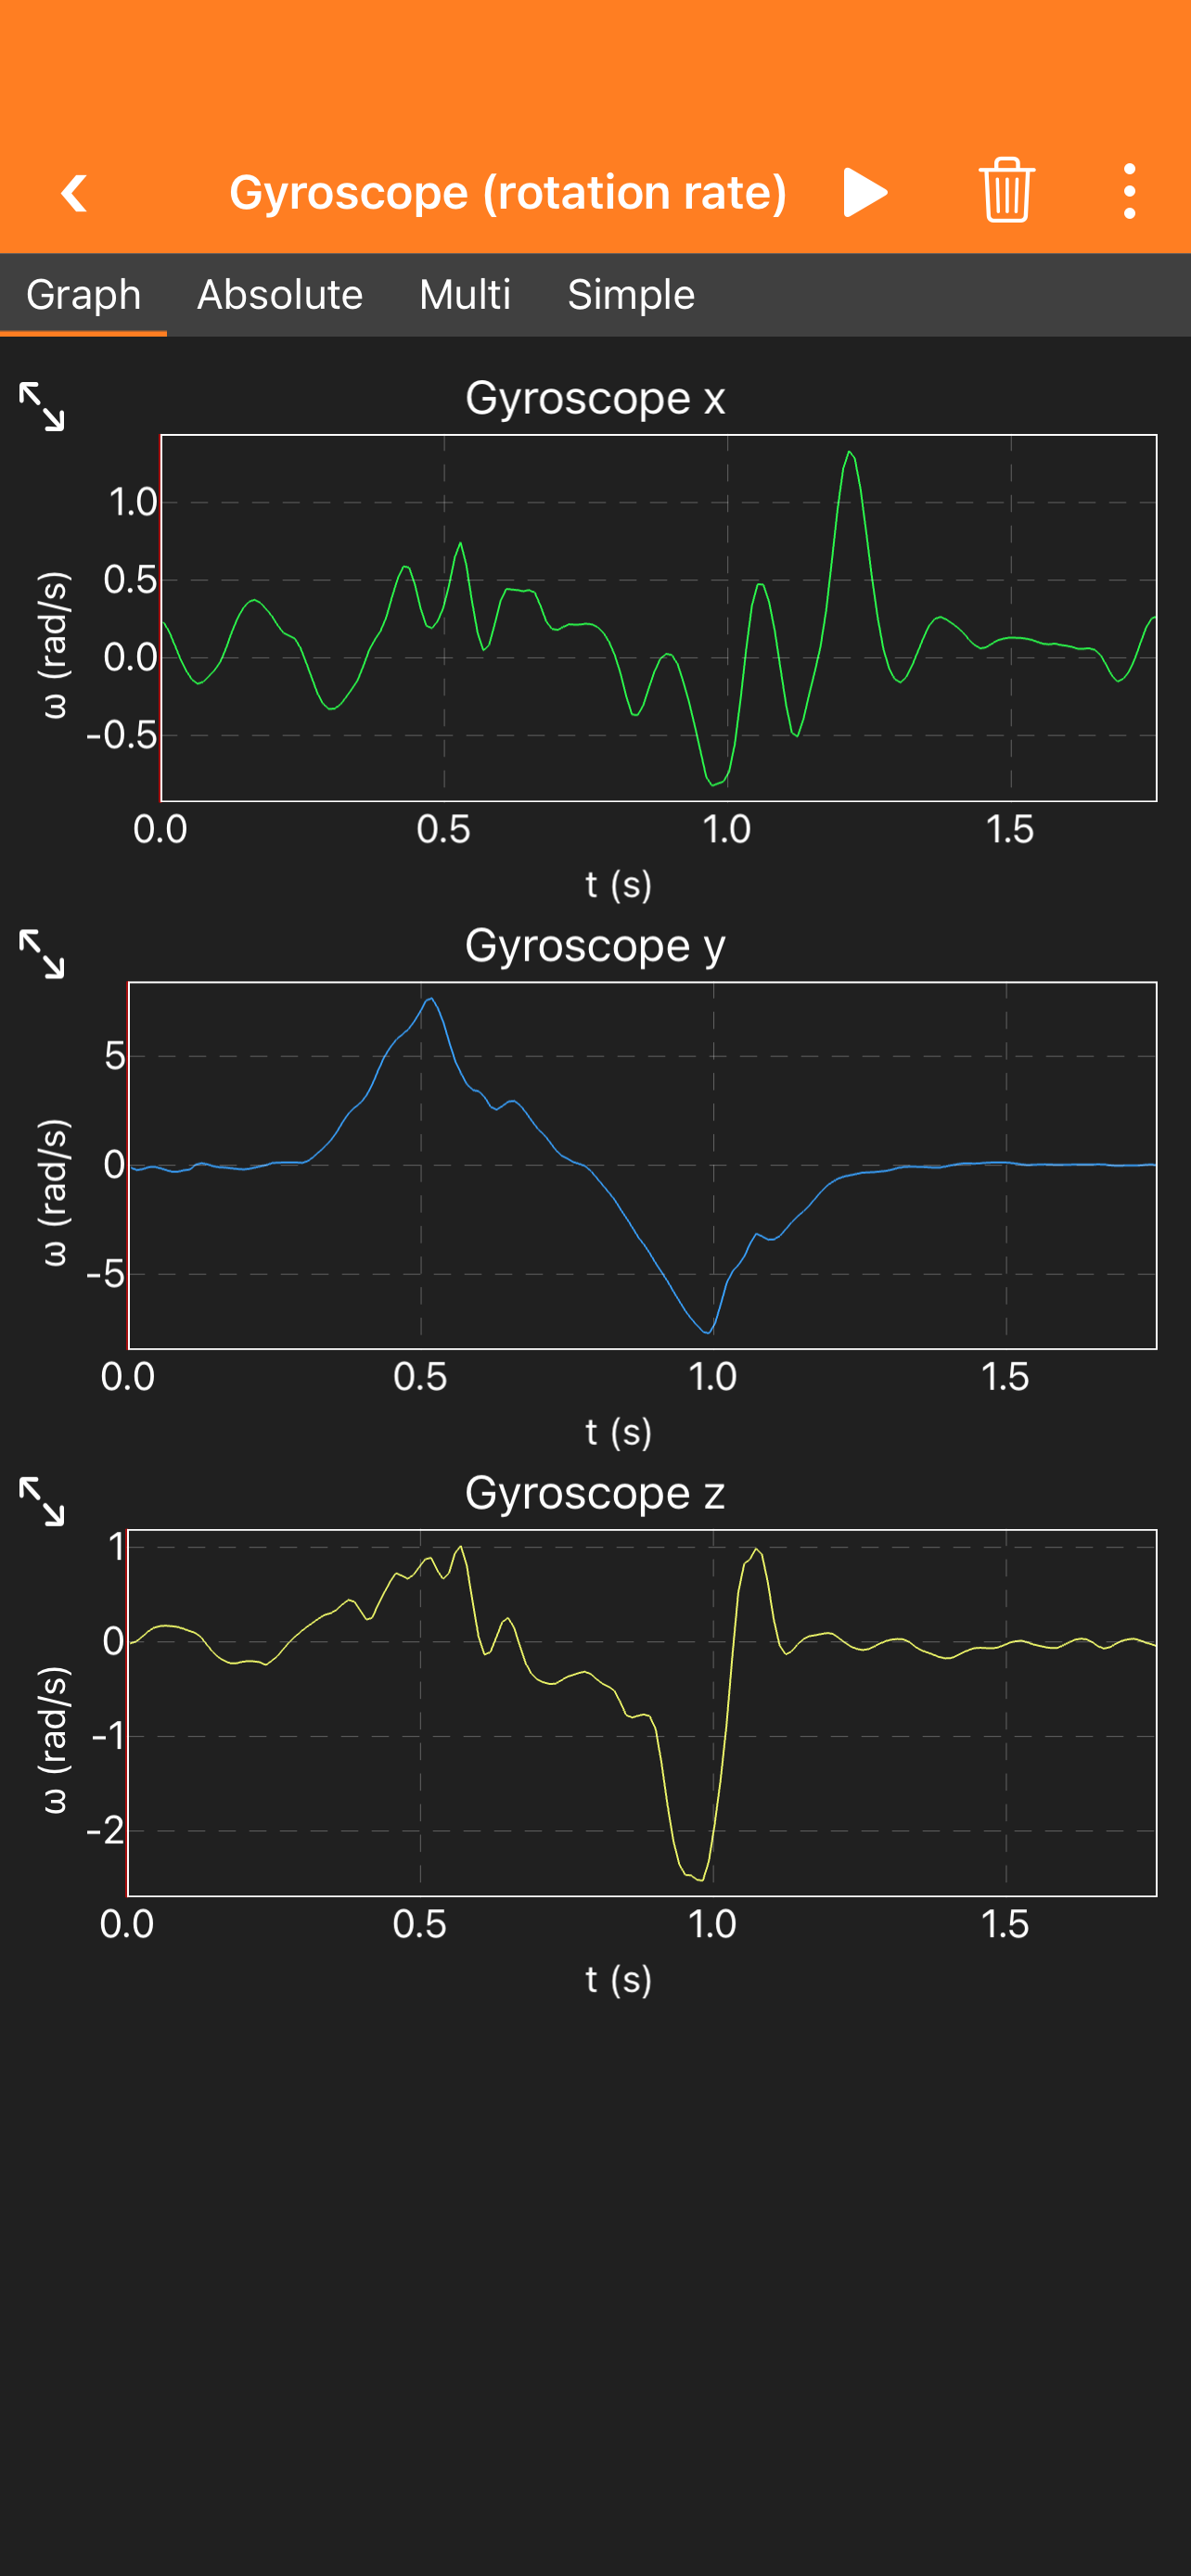
\includegraphics[width=.7\linewidth]{images/Lab.02/GyroscopeY.PNG}
\end{center}
\caption{Screenshot of getting the Gyroscope data for the y-axis for the phone.}
\label{fig:Lab02-GyroscopeY}
\end{figure}

\begin{figure}[H] % Example of including images
\begin{center}
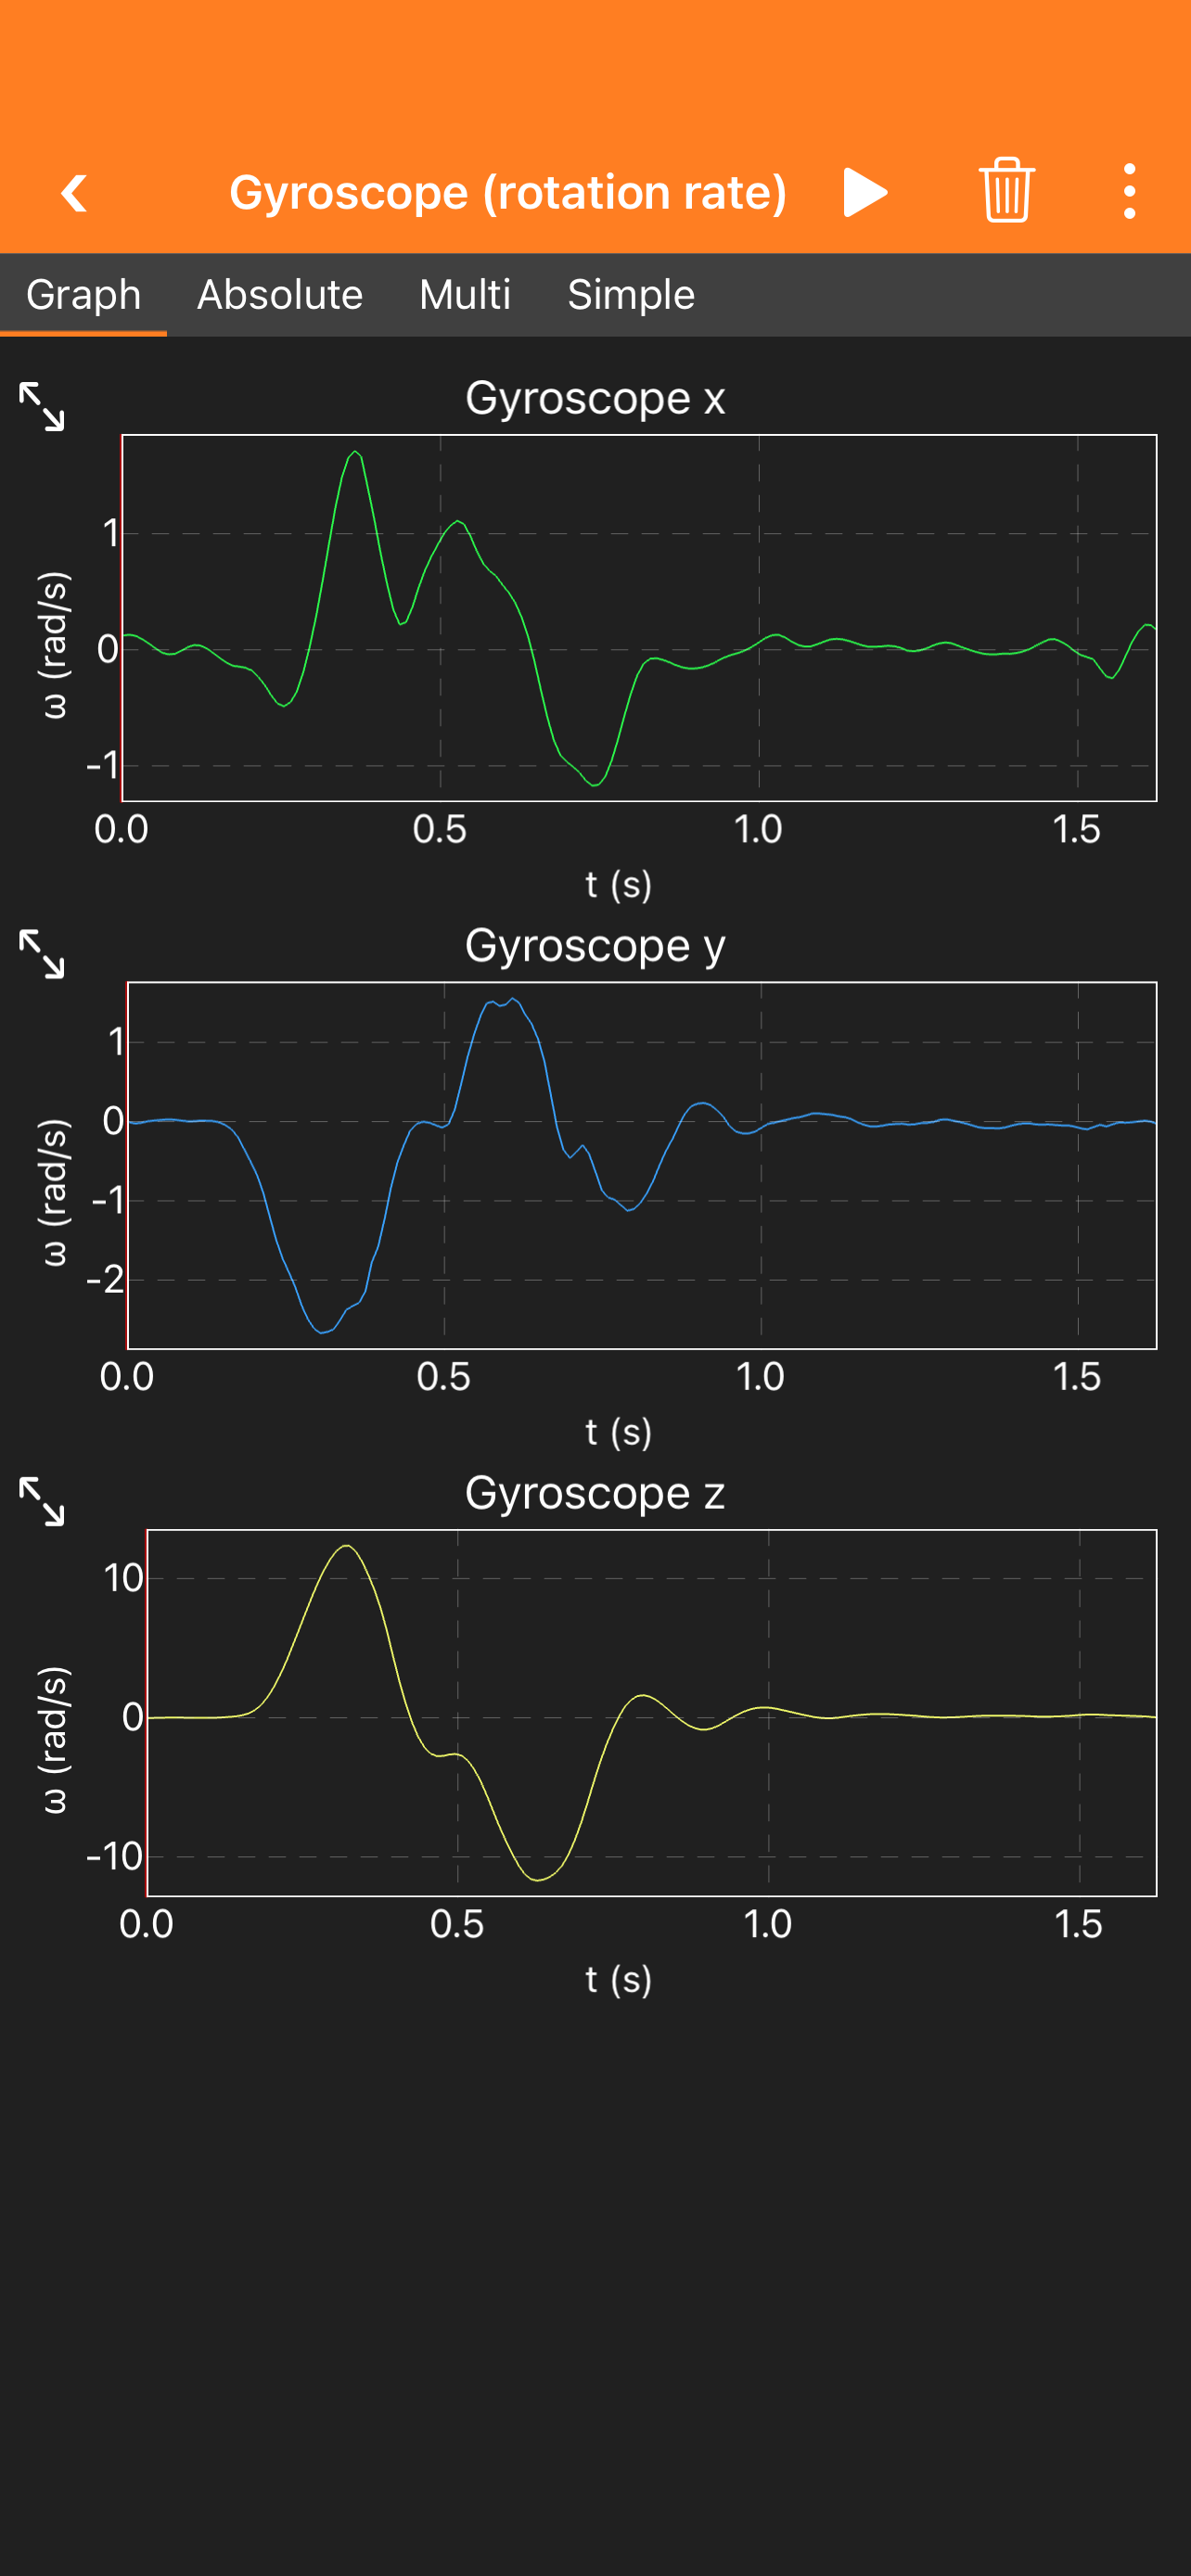
\includegraphics[width=.7\linewidth]{images/Lab.02/GyroscopeZ.PNG}
\end{center}
\caption{Screenshot of getting the Gyroscope data for the z-axis for the phone.}
\label{fig:Lab02-GyroscopeZ}
\end{figure}

%----------------------------------------------------------------------------------------


% \begin{tabular}{l l l l l l l l l l l l l}
% \toprule
% \textbf{Name} & \textbf{Track 1} & \textbf{Track 2} & \textbf{Track 3} & \textbf{Track 4} & \textbf{Track 5} & \textbf{Track 6} & \textbf{Track 7} & \textbf{Track 8} & \textbf{Track 9} & \textbf{Track 10} & \textbf{Track 11} & \textbf{Track 12}    \\
% \toprule
% 1 & 0.2 & 0.8\\
% 2 & 0.17 & 0.7\\
% 3 & 0.24 & 0.75\\
% 4 & 0.68 & 0.3\\
% \bottomrule
% \end{tabular}
% \caption{The effects of treatments X and Y on the four groups studied.}
% \label{tab:treatments_xy}
% \end{table}


%----------------------------------------------------------------------------------------

% \labday{Saturday, Date Month Year}

% \experiment{Bulleted list example} % You don't need to make a \newexperiment if you only plan on referencing it once

% This is a bulleted list:

% \begin{itemize}
% \item Item 1
% \item Item 2
% \item \ldots and so on
% \end{itemize}

% %-----------------------------------------

% \experiment{example}

% \lipsum[6]

% %-----------------------------------------

% \experiment{example2}

% \lipsum[7]

% %----------------------------------------------------------------------------------------
% %	FORMULAE AND MEDIA RECIPES
% %----------------------------------------------------------------------------------------

% \labday{} % We don't want a date here so we make the labday blank

% \begin{center}
% \HRule \\[0.4cm]
% {\huge \textbf{Formulae and Media Recipes}}\\[0.4cm] % Heading
% \HRule \\[1.5cm]
% \end{center}

% %----------------------------------------------------------------------------------------
% %	MEDIA RECIPES
% %----------------------------------------------------------------------------------------

% \newpage

% \huge \textbf{Media} \\ \\

% \normalsize \textbf{Media 1}\\
% \begin{table}[H]
% \begin{tabular}{l l l}
% \toprule
% \textbf{Compound} & \textbf{1L} & \textbf{0.5L}\\
% \toprule
% Compound 1 & 10g & 5g\\
% Compound 2 & 20g & 10g\\
% \bottomrule
% \end{tabular}
% \caption{Ingredients in Media 1.}
% \label{tab:med1}
% \end{table}

% %-----------------------------------------

% %\textbf{Media 2}\\ \\

% %Description

% %----------------------------------------------------------------------------------------
% %	FORMULAE
% %----------------------------------------------------------------------------------------

% \newpage

% \huge \textbf{Formulae} \\ \\

% \normalsize \textbf{Formula 1 - Pythagorean theorem}\\ \\
% $a^2 + b^2 = c^2$\\ \\

%-----------------------------------------

%\textbf{Formula X - Description}\\ \\

%Formula

%----------------------------------------------------------------------------------------

\end{document}